\chapter{Evaluation of Southern Ocean cloud in the HadGEM3 general
circulation model and MERRA-2 reanalysis using ship-based
observations}

\vspace{-0.1cm}\begin{spacing}{1.2}\sffamily\raggedright
Peter~Kuma$^1$, Adrian~J.~McDonald$^1$, Olaf~Morgenstern$^2$, Simon~P.~Alexander$^3$, John~J.~Cassano$^4$, Sally~Garrett$^5$, Jamie~Halla$^5$, Sean~Hartery$^1$, Mike~J.~Harvey$^2$, Simon~Parsons$^1$, Graeme~Plank$^1$, Vidya~Varma$^2$ and~Jonny~Williams$^2$
\end{spacing}

\vspace{0.4cm}\begin{spacing}{1.2}\footnotesize\sffamily\noindent\raggedright
$^1$School of Physical and Chemical Sciences, University of Canterbury, Christchurch, Aotearoa/New Zealand\hfill\break
$^2$National Institute of Water and Atmospheric Research, Wellington, Aotearoa/New Zealand\hfill\break
$^3$Australian Antarctic Division, Kingston, Australia\hfill\break
$^4$Cooperative Institute for Research in Environmental Sciences and Department of Atmospheric and Oceanic Sciences, University of Colorado, Boulder, Colorado,
US\hfill\break
$^5$New Zealand Defence Force, Wellington, Aotearoa/New Zealand
\end{spacing}

\section*{Abstract}

Southern Ocean (SO) shortwave (SW) radiation biases are a common problem in
contemporary general circulation models (GCMs), with most models exhibiting a
tendency to absorb too much incoming SW radiation. These biases have been
attributed to deficiencies in the representation of clouds during the austral
summer months, either due to cloud cover or cloud albedo being too low. The
problem has been the focus of many studies, most of which utilised satellite
datasets for model evaluation. We use multi-year ship based observations and
the CERES spaceborne radiation budget measurements to contrast cloud
representation and SW radiation in the atmospheric component Global Atmosphere
(GA) version 7.1 of the HadGEM3 GCM and the MERRA-2 reanalysis. We find that
the prevailing bias is negative in GA7.1 and positive in MERRA-2. GA7.1
performs better than MERRA-2 in terms of absolute SW bias. Significant errors
of up to 21 \unit{Wm^{-2}} (GA7.1) and 39 \unit{Wm^{-2}} (MERRA-2) are present
in both models in the austral summer. Using ship-based ceilometer observations,
we find low cloud below 2 \unit{km} to be predominant in the Ross Sea and the
Indian Ocean sectors of the SO. Utilising a novel surface lidar simulator
developed for this study, derived from an existing COSP-ACTSIM spaceborne lidar
simulator, we find that GA7.1 and MERRA-2 both underestimate low cloud and fog
occurrence relative to the ship observations on average by 4--9\% (GA7.1) and
18\% (MERRA-2). Based on radiosonde observations, we also find the low cloud
to be strongly linked to boundary-layer atmospheric stability and the sea
surface temperature. GA7.1 and MERRA-2 do not represent the observed
relationship between boundary layer stability and clouds well. We find that
MERRA-2 has a much greater proportion of cloud liquid water in the SO in
austral summer than GA7.1, a likely key contributor to the difference in the SW
radiation bias. Our results suggest that subgrid-scale processes (cloud and
boundary layer parametrisations) are responsible for the bias, and that in
GA7.1 a major part of the SW radiation bias can be explained by cloud cover
underestimation, relative to underestimation of cloud albedo.

\section{Introduction}

Clouds are considered one of the largest sources of uncertainty in estimating
global climate sensitivity \citep{boucher2013,flato2013,bony2015}. Clouds over
oceans are especially important for determining the radiation budget due to the
low albedo of the sea surface compared to land. Over the Southern Ocean (SO),
cloud cover is very high at over 80\%, with boundary-layer clouds being
particularly common \citep{mace2009}. Excess downward shortwave (SW) radiation
in general circulation models (GCMs), with a bias over the SO of up to 30
\unit{Wm^{-2}}, is a problem well-documented by \cite{trenberth2010} and
\cite{hyder2018}, and has been the subject of many studies.
\cite{bodas-salcedo2014} evaluated the SW bias in a number of GCMs and found
that a strong SW bias is a very common feature, leading to increased sea surface
temperature (SST) in the SO and corresponding biases in the storm track
position. \cite{trenberth2010} note that a poor representation of clouds might
lead to unrealistic climate change projections in the Southern Hemisphere. The
SW bias has also been linked to large-scale model problems such as the
double-Intertropical Convergence Zone \citep{hwang2013}, biases in the position
of the midlatitude jet \citep{ceppi2012} and errors in the meridional energy
transport \citep{mason2014}. \cite{bodas-salcedo2012} studied the SO SW bias in
the context of the Global Atmosphere (GA) 2.0 and 3.0,
the atmospheric component of the Hadley Centre Global Environmental Model (HadGEM),
and found that
mid-topped and stratocumulus clouds are the dominant contributors to the bias.

Due to its extent and magnitude, the SW radiation bias is believed to limit 
accuracy of the models, especially for modelling the Southern Hemisphere
climate. A model based on HadGEM3 is currently used in New Zealand for assessing
future climate \citep{williams2016}.
In this paper we evaluate the atmospheric component of HadGEM3, GA7.1
\citep{walters2017} and the reanalysis Modern-Era Retrospective analysis for
Research and Applications, version 2 (MERRA-2) using observations collected in
the SO on a number of voyages. Ship-based atmospheric observations in the SO
provide a unique view of the atmosphere not available via any other means.
Boundary layer observations by satellite instruments are limited by the presence
of an almost continuous cloud cover, potentially obscuring the view of low level
clouds. The frequently used active instruments CloudSat \citep{stephens2002} and
Cloud--Aerosol Lidar and Infrared Pathfinder Satellite Observation (CALIPSO)
\citep{winker2010} are both of limited use when observing low level, thick or
multi-layer cloud: CloudSat is affected by surface clutter below approximately
1.2 \unit{km} \citep{marchand2008} and the CALIPSO lidar signal cannot pass
through thick cloud. Likewise, passive instruments and datasets such as the
Moderate Resolution Imaging Spectroradiometer (MODIS) \citep{salomonson2002} and
the International Satellite Cloud Climatology Project (ISCCP) \citep{rossow1999}
can only observe radiation scattered or emitted from the cloud top of optically
thick clouds. Therefore, one can accurately identify the cloud top height or
cloud top pressure with satellite instruments, but not always the cloud base
height (CBH) or the vertical profile of cloud, although there has been some
recent progress on deriving CBH statistically from CALIPSO measurements
\citep{mulmenstadt2018}. Ship-based measurements therefore provide valuable
extra information.

Multiple explanations of the SW radiation bias have been proposed: cloud
underestimation in the cold sectors of cyclones \citep{bodas-salcedo2014},
cloud--aerosol interaction \citep{vergara-temprado2018}, cloud homogeneity
representation \citep{loveridge2018}, lack of supercooled liquid (cloud liquid
at air temperature below 0$^\circ$C) \citep{kay2016,bodas-salcedo2016} and the
"too few, too bright" problem \citep{nam2012,klein2013,wall2017}. Each model
can exhibit the bias for a different set of reasons, and results from one model
evaluation therefore do not necessarily explain biases in all other models
\citep{mason2015}. The use of SO voyage data for atmospheric model evaluation
is not new, and has recently been used by \cite{sato2018} to evaluate the
impact of SO radiosonde observations on the accuracy of weather forecasting
models. \cite{klekociuk2020} contrasted SO cloud observations with the ECMWF
Interim reanalysis (ERA-Interim) and the Antarctic Mesoscale Prediction
System--Weather Research and Forecasting Model (AMPS-WRF) \citep{powers2012},
and found that these
models underestimate the coverage of the predominantly low cloud.
\cite{protat2017} compared ship-based 95 GHz cloud radar measurements at
43--48$^\circ$S in March 2015 with the Australian Community Climate and
Earth-System Simulator (ACCESS) NWP model, a model related to HadGEM3, and
found low cloud peaking at 80\% cloud cover, which was underestimated in the
model. The clouds were also more spread out vertically (especially due to
"multilayer" situations defined as co-occurrence of cloud below and above 3
km) and more likely to have intermediate cloud fraction rather than very low or
very high cloud fraction. Previous studies have documented that supercooled
liquid is often present in the SO cloud in the austral summer months
\citep{morrison2011,huang2012,chubb2013,huang2016,bodas-salcedo2016,jolly2018,listowski2019}
and is linked to SO SW radiation biases in GCMs, which underestimate the amount
of supercooled liquid in clouds in favour of ice. Warm clouds generally reflect
more SW radiation than cold clouds containing the same amount of water
\citep{vergara-temprado2018}. In particular, \cite{kay2016} reported a
successful reduction of SO absorbed SW radiation in the Community Atmosphere
Model version 5 (CAM5) by decreasing the shallow convection ice detrainment
temperature and thereby increasing the amount of supercooled liquid cloud.

Two common techniques used for model cloud evaluation have been cloud regimes
\citep{williams2009a,haynes2011,mason2014,mason2015,mcdonald2016,jin2017,mcdonald2018,schuddeboom2018,schuddeboom2019}
and cyclone compositing
\citep{bodas-salcedo2012,williams2013,bodas-salcedo2014,bodas-salcedo2016,williams2017},
both of which link the SW radiation bias to specific cloud regimes and cyclone
sectors. We use simple statistical techniques, rather than sophisticated
classification or machine learning algorithms, the advantage of which is easier
interpretation for the purpose of model development.

We first assess the magnitude of the top of the atmosphere (TOA) SO SW radiation
bias in a nudged run of GA7.1 ("GA7.1N") and MERRA-2 with respect to the Clouds
and the Earth's Radiant Energy System (CERES) Energy Balanced and Filled (EBAF)
and CERES Synoptic (SYN) products (Section~\ref{sec:2:sw-radiation-balance}). This
allows us to identify the underlying magnitude of the SW bias and how this might
change based on the ship track sampling pattern. We then evaluate cloud
occurrence in GA7.1N and MERRA-2 relative to the SO ceilometer observations and
compare SO radiosonde observations with pseudo-radiosonde profiles derived from
the models (Sections~\ref{sec:2:cloud-occurrence} and
\ref{sec:2:radiosonde-observations}). Lastly, we look at zonal plots of potential
temperature, humidity, cloud liquid and ice content in GA7.1N and MERRA-2 to
show how these models differ in their atmospheric stability and representation
of clouds (Section~\ref{sec:2:zonal-plane-comparison}). Our aim is to identify how
differences between GA7.1N and MERRA-2 can explain the TOA outgoing SW
radiation bias, assuming misrepresentation of clouds is the major contributor
to the bias.

\begin{table*}[t]
\caption[Table of voyages]{
Table of voyages. The table lists voyages analysed in this study. Listed is  the
voyage name (Voyage), which is the official name of the voyage or an
abbreviation for the purpose of this study, ship name (Ship), organisation
(Org.), start and end dates of the voyage (Start, End), number of days spent at
sea (Days), target region of the SO (Region), maximum and minimum geographical
coordinates of the voyage track (Lat., Lon.). }
\label{tab:2:voyages}
\centering
\centerline{\scalebox{0.8}{
\begin{tabular}[t]{lllllllll}
\hline
\textbf{Voyage} & \textbf{Ship} & \textbf{Org.} & \textbf{Start} & \textbf{End} & \textbf{Days} & \textbf{Region} & \textbf{Lat.} & \textbf{Lon.}\\
\hline
TAN1502 & RV \textit{Tangaroa} & NIWA & 2015-01-20 & 2015-03-12 & 51 & Ross Sea & 41$^\circ$S--75$^\circ$S & 162$^\circ$E--174$^\circ$W\\
TAN1802 & RV \textit{Tangaroa} & NIWA & 2018-02-08 & 2018-03-21 & 41 & Ross Sea & 41$^\circ$S--74$^\circ$S & 170$^\circ$E--175$^\circ$W\\
HMNZSW16 & HMNZS \textit{Wellington} & RNZN & 2016-11-20 & 2016-12-20 & 20 & Ross Sea & 36$^\circ$S--68$^\circ$S & 166$^\circ$E--180$^\circ$E\\
NBP1704 & RV \textit{Nathaniel B. Palmer} & NSF & 2017-04-11 & 2017-06-13 & 63 & Ross Sea & 53$^\circ$S--78$^\circ$S & 163$^\circ$E--174$^\circ$W\\
AA15 (AA V1--V3) & \textit{Aurora Australis} & AAD & 2015-10-22 & 2016-02-22 & 123 & Indian O. sector & 42$^\circ$S--69$^\circ$S & 62$^\circ$E--160$^\circ$E\\
\hline
\end{tabular}
}}
\end{table*}

\section{Datasets}
\label{sec:2:datasets}

We used an observational dataset of ceilometer and radiosonde data comprising
multiple SO voyages (Section~\ref{sec:2:ship-observations}), GA7.1N atmospheric
model simulations (Section~\ref{sec:2:hadgem3}) and the MERRA-2 reanalysis
(Section~\ref{sec:2:merra-2}). Later in the text, we will refer to GA7.1N and
MERRA-2 together as "the models", even though MERRA-2 is more specifically a
reanalysis. CERES satellite observations \citep{wielicki1996} were also used as
a reference for TOA outgoing SW radiation and an National Snow and Ice Data
Center (NSIDC) satellite-based dataset \citep{maslanik1999} was used as an
auxiliary dataset for identifying sea ice.

\subsection{Ship observations}
\label{sec:2:ship-observations}

\begin{figure*}[t]
\centering
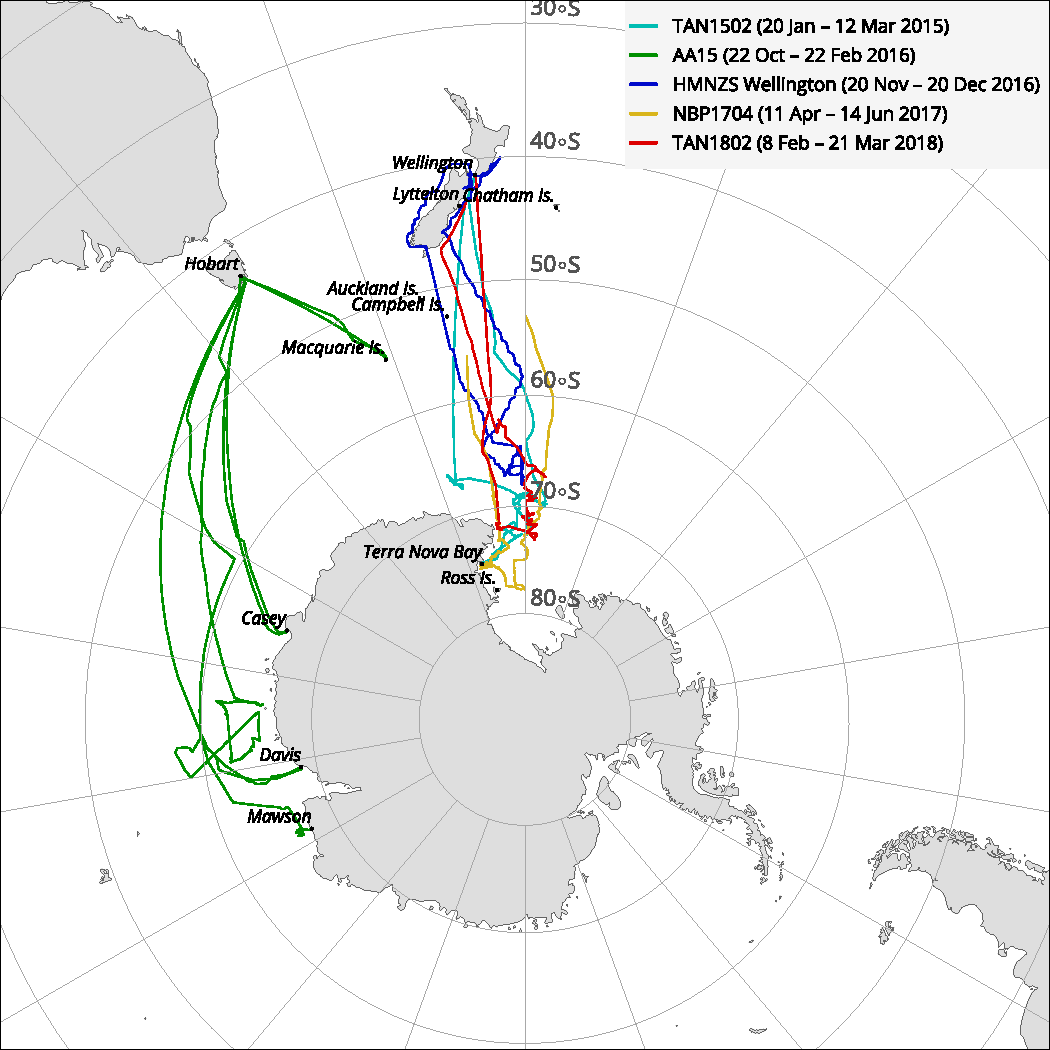
\includegraphics[width=0.75\textwidth]{chapter2/fig/map_rev2.pdf}
\caption[Map showing tracks of voyages]{
Map showing tracks of voyages used in this study. The ship observational dataset
comprises 5 voyages between 2015 and 2018, spanning months from November to June
and latitudes between 40$^\circ$S and 78$^\circ$S, of which data between
50$^\circ$S and 70$^\circ$S are used in this study.
}
\label{fig:2:map}
\end{figure*}

We use ship-based ceilometer and radiosonde observations made in the SO on 5
voyages between 2015 and 2018 (Table~\ref{tab:2:voyages} and Fig.
\ref{fig:2:map}):\footnote{The voyage name pattern is a 2--6 character ship name
followed by a 2 digit year and a 2 digit sequence number. TANxxxx and NBPxxxx
are official voyage names, while HMNZSW16 and AA15 are names made for the
purpose of this study.}

\begin{itemize}
\item 2015 TAN1502 voyage of the NIWA ship RV \textit{Tangaroa} from Wellington,
New Zealand to the Ross Sea.
\item 2015--2016 voyages (V1--V3) of the Australian Antarctic Division (AAD)
icebreaker \textit{Aurora Australis} from Hobart, Australia to Mawson, Davis,
Casey and Macquarie Island ("AA15")
\item 2016 Royal New Zealand Navy (RNZN) ship HMNZS \textit{Wellington} voyages
("HMNZSW16").
\item 2017 NBP1704 voyage of the NSF icebreaker RV \textit{Nathaniel B. Palmer}
from Lyttelton, New Zealand to the Ross Sea.
\item 2018 TAN1802 voyage of RV \textit{Tangaroa} from Wellington to the Ross
Sea \citep{hartery2019}.
\end{itemize}

Together, these voyages cover latitudes between 41 and 78$^\circ$S and the
months of November to June inclusive. A total of 298 days of observations were
collected. Geographically, the voyages mostly cover the Ross Sea sector of the
SO, with only AA15 covering the Indian Ocean sector (Fig.~\ref{fig:2:map}). This
sampling emphasises the Ross Sea sector over other parts of the SO, although the
SO SW radiation bias is present at all longitudes in the SO (Section
\ref{sec:2:sw-radiation-balance}), affected by the atmospheric circulation
\citep{jones1993,sinclair1994,sinclair1995,simmonds2000,simmonds2003,simmonds2003a,hoskins2005,hodges2011}.
The voyage observations were performed using a range of instruments (described
below). Table~\ref{tab:2:deployments} details which instruments were deployed on
each voyage.

\begin{table*}[t]
\caption[Table of deployments]{
Table of deployments. The table cells indicate if data from a given instrument
(row) was available from a voyage (column).
}
\label{tab:2:deployments}
\centering
\begin{tabular}[t]{lccccc}
\hline
Instrument/Voyage & AA15 & TAN1502 & HMNZSW16 & NBP1704 & TAN1802\\
\hline
Lufft CHM 15k & & & \checkmark & \checkmark & \checkmark\\
Vaisala CL51 & \checkmark & \checkmark & & & \\
iMet radiosondes & & & & & \checkmark\\
Radiosondes (other) & & & & \checkmark & \\
\hline
\end{tabular}
\end{table*}

The primary instruments were the Lufft CHM 15k and Vaisala CL51 ceilometers. A
ceilometer is an instrument which typically uses a single-wavelength laser to
emit pulses vertically into the atmosphere and measures subsequent backscatter
resolved on a large number of vertical levels based on the timing of the
retrieved signal \citep{emeis2010}. Depending on the wavelength, the emitted
signal interacts with cloud droplets, ice crystals and precipitation by Mie
scattering, and to a lesser extent with aerosol and atmospheric gases by
Rayleigh scattering \citep{bohren2008}. The signal is quickly attenuated in
thick cloud and therefore it is normally not possible to observe mid and high
level parts of such a cloud, or a multi-layer cloud. The main derived quantity
determined from the backscatter is CBH, but it is also possible to apply a cloud
detection algorithm to determine cloud occurrence by height. The
range-normalised signal is affected by noise which increases with the square of
range. A major source of noise is solar radiation which causes a diurnal
variation in noise levels \citep{kotthaus2016}. Due to signal attenuation and
noise ceilometers cannot measure clouds obscured by a lower cloud, and therefore
cannot be used for 1:1 comparison with model clouds without using a lidar
simulator, which accounts for this effect \citep{chepfer2008}. The Lufft CHM 15k
ceilometer operates in the near-infrared spectrum at 1064 nm, measuring lidar
backscatter up to a maximum height of 15 \unit{km}, producing 1024 regularly
spaced bins (about 15 m resolution). The sampling rate of the instrument is 2
\unit{s}. The Vaisala CL51 ceilometer operates in the near-infrared spectrum at
910 nm. The sampling rate of the instrument is 2 \unit{s} and range is 7.7
\unit{km}, producing 770 regularly spaced bins (10 m resolution).

Radiosonde observations were performed on the TAN1802 and NBP1704 voyages south
of 60$^\circ$S.  Temperature, pressure, relative humidity and Global Navigation
Satellite System (GNSS) coordinates
(from which wind speed and direction are derived) were retrieved to altitudes
of about 10--20 \unit{km}, terminated by a loss of radio communication or
balloon burst.
On the TAN1802 voyage we used iMet-1 ABx radiosondes.
The sondes were launched three
times per day at about 8:00, 12:00 and 20:00 UTC on 100 \unit{g} Kaymont
weather balloons.We used 10
\unit{s} resolution profiles generated by the vendor-supplied iMetOS-II control
software for further processing.

Automatic weather station (AWS) data were available on the TAN1502, TAN1802 and
NBP1704 voyages. These included variables such as air temperature, pressure,
sea surface temperature, wind speed and wind direction. Voyage track
coordinates were obtained from the ships' GNSS receivers.

\subsection{HadGEM3}
\label{sec:2:hadgem3}
HadGEM3 \citep{walters2017} is a general circulation model developed by the UK
Met Office and the Unified Model Partnership.
It can be used in a "nudging" \citep{telford2008} mode, in which winds and
potential temperature are relaxed towards the ERA-Interim reanalysis
\citep{dee2011}. The Met Office Global Atmosphere 7.1 (GA7.1) is the atmospheric
component of HadGEM3 \citep{walters2017}, based on the Unified Model (UM)
version 11.0.

The model runs used the HadISST sea surface temperature dataset
\citep{rayner2003} as lateral boundary conditions. The nudged simulations
represent atmospheric dynamics as determined by observations. The model was run
on a 1.875$^\circ$$\times$1.25$^\circ$ (longitude $\times$ latitude) "N96"
resolution grid, which corresponds to a horizontal resolution of about
100$\times$140 \unit{km} at 60$^\circ$S and 85 vertical levels. The model output
fields were sampled every 6 hours (instantaneous) and daily (mean). In our
analysis we used a nudged run of GA7.1 ("GA7.1N") between years 2015 and 2018,
corresponding to the ship observations.

\subsection{MERRA-2}
\label{sec:2:merra-2}

Modern-Era Retrospective analysis for Research and Applications (MERRA-2) is a
reanalysis provided by the NASA Global Modelling and Assimilation Office
\citep{gelaro2017}. The reanalysis was chosen for its contrasting results of
TOA outgoing SW radiation bias in the SO compared to GA7.1. As shown later
(Fig.~\ref{fig:2:sw_up_toa_geo}), its bias is positive rather than negative,
when CERES is used as a reference.

We used the following products \citep{bosilovich2015}:

\begin{itemize}
\item 1-hourly average Radiation Diagnostics (product "M2T1NXRAD.5.12.4")
\item 3-hourly instantaneous Assimilated Meteorological Fields (product
"M2I3NVASM.5.12.4")
\item 1-hourly instantaneous Single-Level Diagnostics (product
"M2I1NXASM.5.12.4")
\item 3-hourly average Assimilated Meteorological Fields (product
"M2T3NVASM.5.12.4")
\item 1-hourly average Single Level Diagnostics (product "M2T1NXSLV.5.12.4")
\end{itemize}

We used the "Radiation Diagnostics" in TOA outgoing SW radiation evaluation (Section
\ref{sec:2:sw-radiation-balance}), the instantaneous "Assimilate Meteorological
Fields" and "Single-Level Diagnostics" products to generate simulated
ceilometer profiles and pseudo-radiosonde profiles (Section
\ref{sec:2:cloud-occurrence} and~\ref{sec:2:radiosonde-observations}), and the
average "Assimilate Meteorological Fields" and "Single-Level Diagnostics" to
generate zonal plane plots of thermodynamic and cloud fields (Section
\ref{sec:2:zonal-plane-comparison}). The 4-dimensional MERRA-2 fields were
provided on pressure and model levels. For our analysis we chose to use the
model-level products (72 levels) due to their higher vertical resolution
compared to pressure-level products. The analysed time period of MERRA-2 data
was 2015--2018.

\subsection{CERES}

The Clouds and the Earth's Radiant Energy System (CERES) is a set of low Earth
orbit (LEO) satellite instruments and a dataset of SW and longwave (LW)
radiation observations \citep{loeb2018,doelling2016}. The CERES instruments
(called FM1 to FM6) provide a continuous record of observations since the first
deployment on the Tropical Rainfall Measuring Mission (TRMM) satellite in 1997
\citep{simpson1996}, and have been flown on Terra, Aqua \citep{parkinson2003},
the Suomi NPOESS Preparatory Project (Suomi NPP) and Joint Polar Satellite
System-1 (JPSS-1) \citep{goldberg2013} satellites since. Currently CERES is
considered the best available global Earth radiation datasets, and is often used
as the primary dataset for GCM tuning and validation
\citep{schmidt2017,hourdin2017}. We used the following CERES products in our
analysis:

\begin{itemize}
\item CERES SYN1deg-Day Edition 4A (configuration code 406406 and 407406)
product of daily average radiation ("CERES SYN").
\item CERES EBAF-TOA Edition 4.1 (CERES\_EBAF\_Ed4.1)
product of monthly energy-balanced average radiation ("CERES EBAF").
\end{itemize}

Due to the sun-synchronous orbits of the LEO satellite platforms, the Flight
Model (FM) instruments of CERES do not capture the full diurnal variation of
radiation. The EBAF and and SYN1deg products are adjusted for diurnal variation
by using 1-hourly geostationary satellite observations between 60$^\circ$S and
60$^\circ$N, and use an algorithm to account for changing solar zenith angle and
diurnal land heating. The CERES EBAF-TOA Edition 4.1 product is a Level 3B
product, which means it has been globally balanced by ocean heat measurements
using the Argo network \citep{roemmich2009a,roemmich2009b}.

\subsection{NSIDC sea ice concentration}

We used the Near-Real-Time Defense Meteorological Satellite Program (DMPS)
Special Sensor Microwave Imager/Sounder (SSMIS) Daily Polar Gridded Sea Ice
Concentrations, Version 1 product (NSIDC-0081) \citep{maslanik1999} provided by
the National Snow and Ice Data Center (NSIDC) to classify observations into
those affected and unaffected by sea ice. The sea ice concentration product has
a resolution of 25$\times$25 \unit{km}. We used a cutoff value of 15\% of sea
ice concentration for the binary classification of sea ice, in line with
previous studies \citep{comiso2008}.

\begin{figure*}[t]
\centering
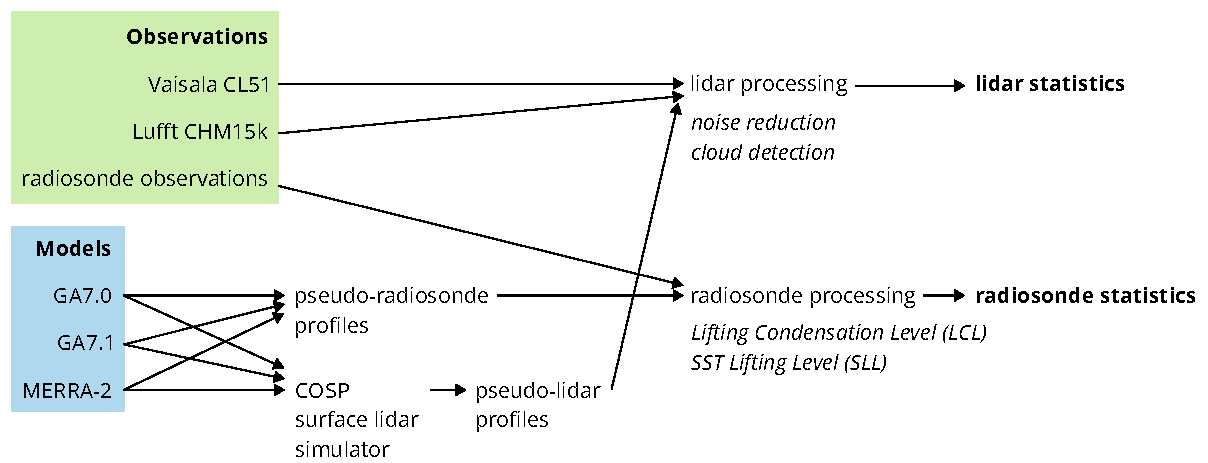
\includegraphics[width=\textwidth]{chapter2/fig/schematic.pdf}
\caption[Schematic of the processing pipeline]{
Schematic of the processing pipeline utilised in this study to produce lidar and
radiosonde statistics from observations and model data.
}
\label{fig:2:schematic}
\end{figure*}

\section{Methods}

\subsection{Lidar simulator}

CFMIP Observation Simulator Package (COSP) \citep{bodas-salcedo2011}, a set of
instrument simulators developed by the Cloud Feedback Model Intercomparison
Project (CFMIP), was extended with a surface lidar simulator and used to produce
virtual lidar measurements from model fields \citep{kuma2020b}. Resampling, noise
reduction and cloud detection were performed on observational and (where
applicable) model lidar data in a consistent way to reduce structural
uncertainty (see Section~\ref{sec:2:lidar-data-processing}). The schematic in
Fig.~\ref{fig:2:schematic} shows the processing pipeline utilised in this study.

COSP was originally developed as a satellite simulator package whose aim is to
produce virtual satellite (and more recently ground-based) observations from
atmospheric model fields in order to improve comparisons of model output with
observations \citep{bodas-salcedo2011}. This approach is required because
physical quantities derived from satellite observations generally do not
directly correspond to model fields. COSP accounts for the limited view of the
satellite instrument by calculating radiative transfer through the atmosphere,
i.e. attenuation by hydrometeors and air molecules and backscattering. COSP
comprises multiple instrument simulators, such as MODIS, ISCCP, MISR, CALIPSO
and CloudSat. It has been used extensively by previous studies of model cloud,
for example by \cite{kay2012}, \cite{franklin2013}, \cite{klein2013},
\cite{williams2017}, \cite{jin2017} , and \cite{schuddeboom2018}. COSP is
planned to be used in the upcoming Coupled Model Intercomparison Project Phase 6
(CMIP6) \citep{webb2017}.

For our analysis, we have developed a ground-based lidar simulator by modifying
the COSP ACTSIM spaceborne lidar simulator \citep{chiriaco2006} (see
the Code and data availability section at the end of the document). This
required reversing of the vertical layers, as the surface lidar looks from the
surface up rather than down from space to the surface, and changing the
radiation wavelength affecting Mie scattering by cloud droplets and Rayleigh
scattering by air molecules. In this paper we present only a brief description
of the surface lidar simulator, with a more complete description planned in an
upcoming paper. The new simulator is made available as part of the Automatic
Lidar and Ceilometer Framework (ALCF) at \url{https://alcf-lidar.github.io}.

The recently introduced COSP version 2 \citep{swales2018} added support for a
surface lidar simulator, although we believe our implementation, developed
before COSPv2 was available, is more complete in the present context due to its
treatment of Mie scattering at wavelengths other than 532 nm (the wavelength of
the CALIPSO lidar). Previously, a surface lidar simulator based on COSP has
been used by \cite{chiriaco2018} and \cite{bastin2018}. A ground-based radar
simulator in COSP has also recently been implemented \citep{zhang2018}. 

The surface lidar simulator takes model cloud liquid and ice mixing ratios,
cloud fraction and thermodynamic profiles as the input, and calculates vertical
profiles of attenuated backscatter. This can be done either by running the
simulator "online" within the model code or "offline" on the model output.
We used the offline approach in our analysis.

\subsection{Lidar data processing}
\label{sec:2:lidar-data-processing}

Lidar data in this study came from two different instruments: Lufft CHM 15k and
Vaisala CL51 ceilometers and the lidar simulator. These instruments use
different output formats, wavelengths, sampling rates and range bins, as
previously noted. Backscatter and derived fields such as CBH are provided in the
firmware generated data products, but the backscatter is uncalibrated and the
derived fields such as cloud detection are based on instrument-dependent
algorithms. Therefore, we performed consistent subsampling, noise reduction and
cloud detection on data from both instruments, and applied the same methods to
the lidar simulator output. As part of the processing we developed a publicly
available tool called cl2nc ("CL to NetCDF") for converting the Vaisala CL51
ceilometer data format to NetCDF (see the Code and data availability section at
the end of the document).

\subsubsection{Calibration}
\label{sec:2:calibration}

The backscatter profiles produced by the Lufft CHM 15k and Vaisala CL51
ceilometers are not calibrated to physical units, even though they are expressed
in \unit{m^{-1} sr^{-1}}. To calibrate these backscatter fields we used the
method described by \cite{oconnor2004}. This method uses the lidar ratio (LR) to
calculate a calibration factor based on a known value of the LR in fully
scattering cloudy scenes (18.8 $\pm$ 0.8 \unit{sr}), such as thick stratocumulus
clouds, which are common over the SO. We applied this technique by using
visually identified scenes and choosing a calibration factor which achieves the
known value. Due to the nature of the conditions (LR can be highly variable even
in thick cloud scenes), the calibration is likely accurate to only about 50\% of
the backscatter value. We do not expect this to have a serious impact on the
accuracy of cloud detection completed in this study, largely because the
predominantly low cloud tends to cause backscatter orders of magnitude greater
than clear air, and because of the very large differences in cloud occurrence
between the observations and models.

\subsubsection{Subsampling, noise removal and cloud detection}
\label{sec:2:subsampling}

In order to simplify further processing and increase the signal-to-noise ratio,
we subsampled the ceilometer observations at a sampling rate of 5 minutes by
averaging multiple profiles, and vertically averaging on regularly spaced 50
\unit{m} bins. We expect that in most cases cloud was almost constant on this
time and vertical scale, and therefore we were not averaging together different
cloud types or clear and cloudy profiles. At the same time as subsampling, we
performed noise removal by estimating the noise distribution (mean and standard
deviation) based on returns in the uppermost range bins (i.e. 300 samples over 5
min when sampling rate was 2 \unit{s}), and subtracting the range-scaled noise
mean from the backscatter. We then used the range-scaled noise standard
deviation ($\sigma$) for cloud detection: a bin was considered cloudy if the
calibrated backscatter minus 3$\sigma$ exceeded 20$\times$10$^{-6}$ \unit{m^{-1}
sr^{-1}}. This threshold was chosen subjectively so that cloud was visually well
separated from other features, such as boundary-layer aerosol and noise on
backscatter profile plots. The same threshold was used on both the observations
and output from the COSP surface lidar simulator and thus should cause little
bias.

\subsubsection{Model lidar data processing}

We used the same sampling rate (5 min) and model levels as range bins on the
surface lidar simulator output. For each vertical profile we used model data at
the same location as the ship and the same time relative to the start of the
year. Model data were selected using nearest-neighbour interpolation. The model
resolution is lower than the distance travelled by the ship in 5 minutes,
therefore the same model data were used multiple times to generate consecutive
profiles. However, we also used the SCOPS \citep{webb2001} subcolumn generator
included in COSP to generate 10 random samples of cloud for each profile based
on cloud fraction and the maximum/random cloud overlap assumption \citep{cosp}.
The lidar simulator processes each sample individually. The resulting cloud
occurrence is calculated as the average of the 10 samples. The lidar simulator
does not generate noise, and therefore we did not perform any noise removal on
the simulated profiles, but we used the same threshold of 20$\times$10$^{-6}$
\unit{m^{-1} sr^{-1}} and vertical bins of 50 m for detecting cloud (as used on
the observations). For the MERRA-2 cloud occurrence analysis, we applied the
lidar simulator on the 3-hourly instantaneous Assimilated Meteorological Fields
(M2I3NVASM.5.12.4) product.

\section{Spatiotemporal subsets investigated}
\label{sec:2:domains}

Because our observational dataset does not span the entire geographical area of
the SO and all months of the year, and the atmospheric conditions in the SO are
geographically variable, we subset the datasets into a number of geographical
regions by latitude and time periods by season. The geographical regions
investigated are 50--75$^\circ$S by 5 degrees of latitude, and the temporal
periods investigated are austral summer of December, January, February (DJF)
and autumn months of March, April, May (MAM).

We do not use data from 70--75$^\circ$S and 50--55$^\circ$S in all parts of
the analysis.  The data from 70--75$^\circ$S are likely affected by
circulation induced by land near the Ross Sea \citep{coggins2014}, and
therefore may not be representative of the SO in general. This decision builds
on the analysis detailed in \cite{jolly2018} which shows a significant gradient
in cloud properties between the Ross Ice Shelf and the Ross Sea and strong
influences associated with synoptic conditions. The data from 50--55$^\circ$S
were relatively sparse (the ships spent relatively little time passing through
this latitudes). Radiosonde observations were only available south of
60$^\circ$S.

There is likely temporal variability present within the DJF and MAM
time periods, but we decided to limit the number of temporal subsets
to maintain a reasonable quantity of observations in each subset.
The magnitude of the SO TOA outgoing SW radiation bias is primarily modulated
by incoming solar radiation, which is the highest in DJF.
The voyages do not uniformly cover all geographical regions or time periods,
with the largest number of observations in the Ross Sea sector south of New
Zealand (TAN1802, TAN1502, HMNZSW16, NBP1704), followed by the Indian Ocean
sector south of Western Australia (AA15). Temporally, the voyage observations
mostly cover summer to autumn months of the year.

\section{Results}

\subsection{Shortwave radiation balance}
\label{sec:2:sw-radiation-balance}

\begin{figure*}[t]
\centering
\centerline{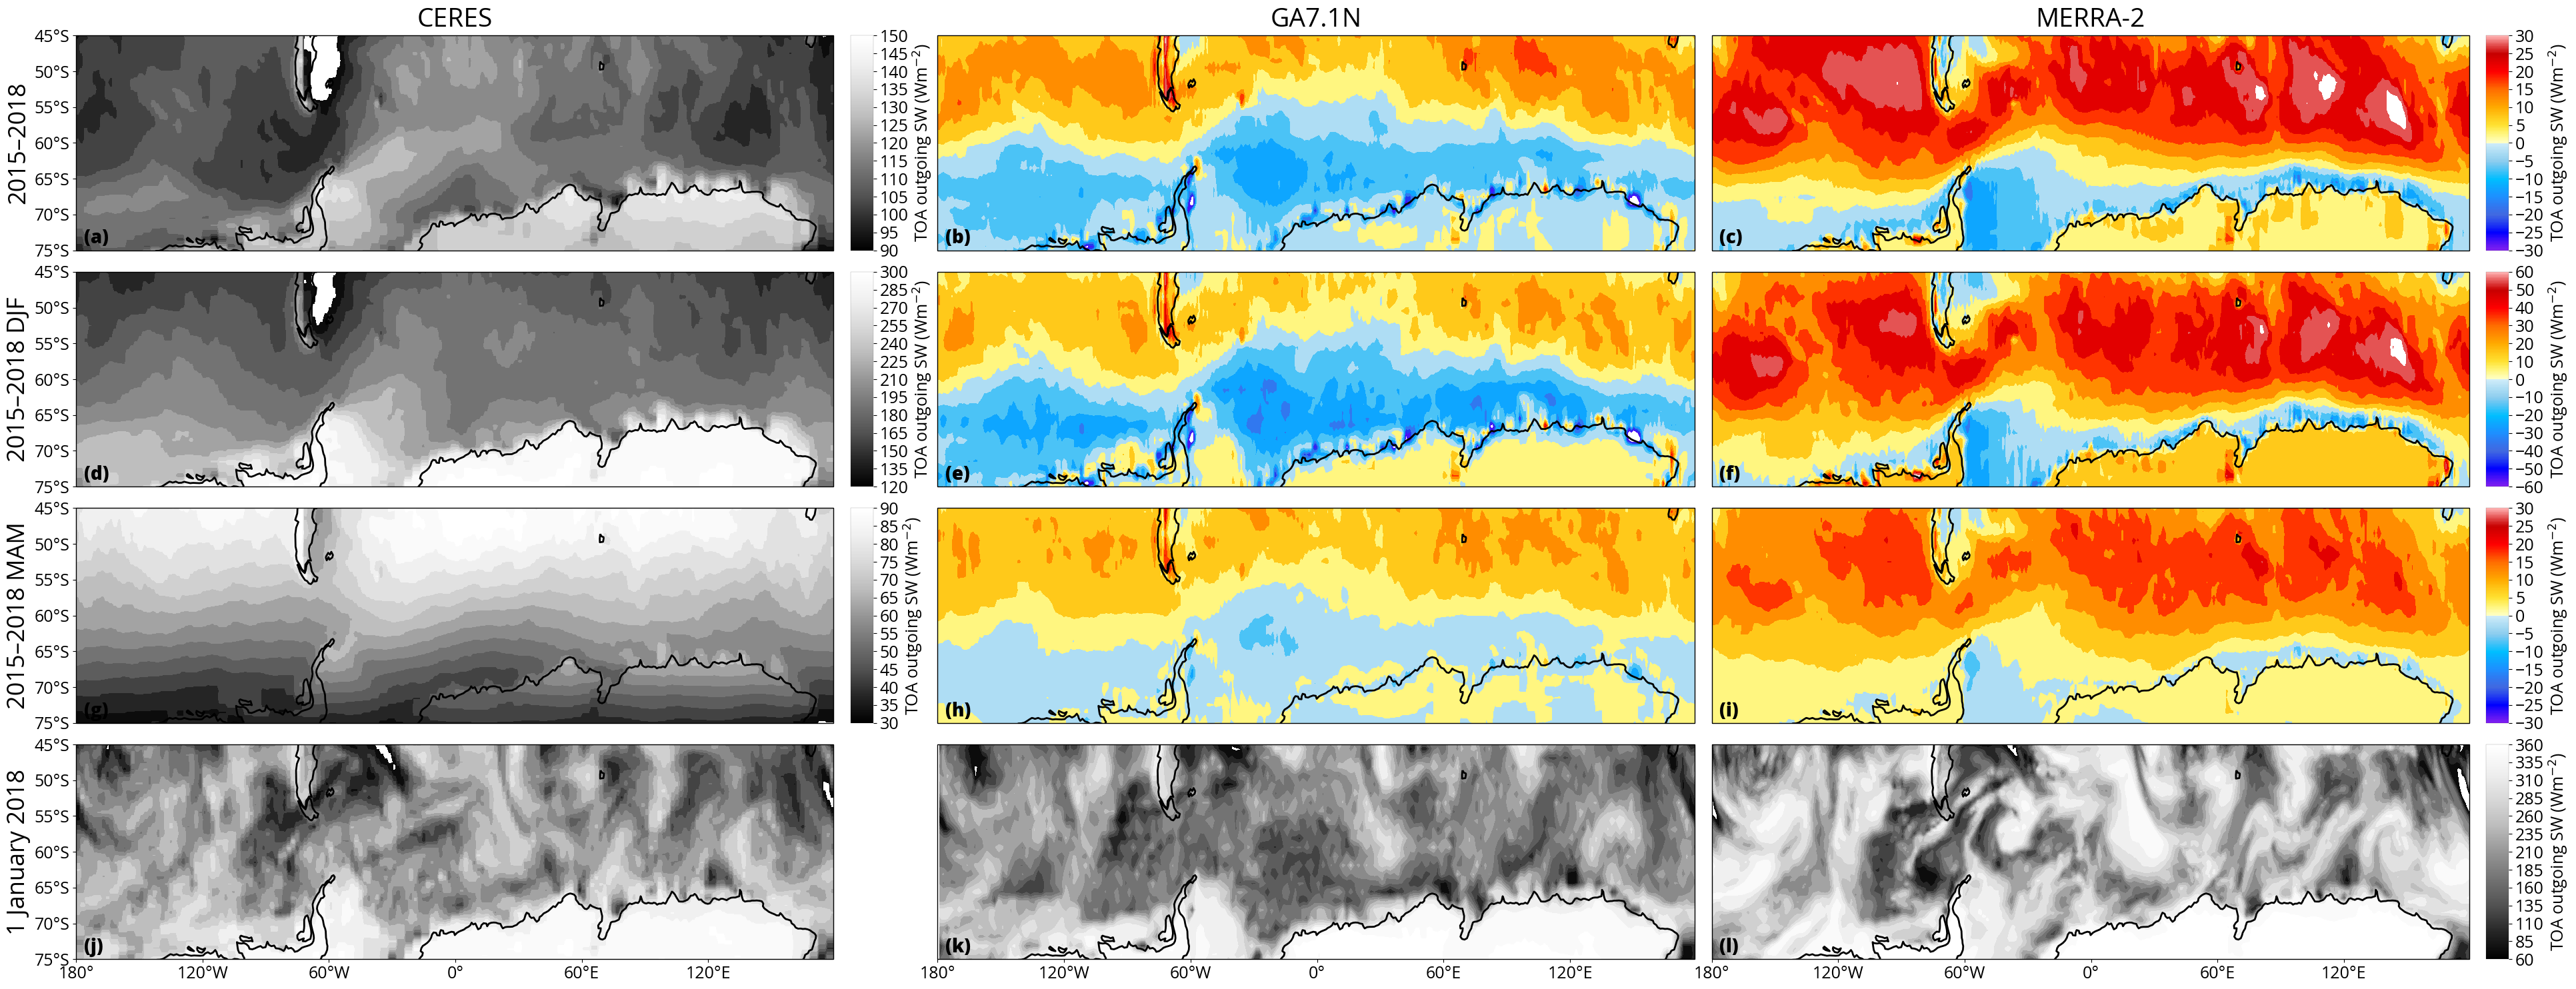
\includegraphics[width=1.12\textwidth]{chapter2/fig/sw_up_toa_geo_rev1.png}}
\caption[Geographical distribution of the TOA outgoing SW radiation in CERES, GA7.1N and
MERRA-2]{
Geographical distribution of the TOA outgoing SW radiation in CERES, GA7.1N and
MERRA-2. The plots show\ global all sky SW radiation as annual (2015--2018;
\textbf{a--c}), seasonal (2015--2018 DJF, MAM; \textbf{d--i}) and daily (1 January 2018; \textbf{j--l})
mean. The blue--red colormap shows bias relative to CERES \textbf{(b, c, e, f, h, i)},
while the grayscale colormap shows absolute values \textbf{(a, d, g, j, k, l)}.
}
\label{fig:2:sw_up_toa_geo}
\end{figure*}

Figure~\ref{fig:2:sw_up_toa_geo} shows TOA outgoing SW radiation in CERES, GA7.1
and MERRA-2. We present this panel plot in order to evaluate how well GA7.1N and
MERRA-2 are performing in terms of SW radiation bias in the SO relative to
CERES. This analysis assumes that CERES is a good observational reference,
although it is affected by errors of lower order of magnitude (2.5 Wm$^{-2}$
"regional monthly uncertainty" \citep[Sect. 4a]{loeb2018}). The plots reveal
relatively zonally symmetric pattern of negative and positive bias on the
annual (Fig.~\ref{fig:2:sw_up_toa_geo}b, c) and seasonal (Fig.
\ref{fig:2:sw_up_toa_geo}e, f, h, i) time scales. GA7.1N shows predominantly
negiative bias, while MERRA-2 shows predominantly positive bias. The annual
average is dominanted by the bias in DJF due to the relatively strong incoming
solar radiation in DJF. The bias displays very similar geographical pattern on
the annual scale, DJF and MAM. The bias is much lower in MAM compared to DJF
due to lower incoming solar radiation.

We chose 1 January 2018 as a representative day in DJF to show the daily scale.
On the daily scale (Fig.~\ref{fig:2:sw_up_toa_geo}j, k, l), the patterns are
closely linked to synoptic features. The region on the eastern side of the
Antarctic Peninsula shows the greatest negative bias in the models. The
relatively zonally symmetric annual and seasonal means suggest that there is
not a significant need for subsetting by longitude, and that latitude averages
can be very useful in identifying the key features of the SW radiation biases.
The daily synoptic features are generally well-correlated between CERES and the
models, which is expected in nudged model runs and reanalyses. MERRA-2 has
greater TOA outgoing SW radiation than GA7.1N on all three time periods
presented here. Considering that cloud is the dominant factor affecting SW
radiation in the SO (apart from sea ice, which is prescribed in MERRA-2 based on observations), this can only be associated with either cloud cover which
is too high, or cloud albedo which is too high. GA7.1N reflects too little SW
radiation south of 60$^\circ$S and too much north of 60$^\circ$S (Fig.
\ref{fig:2:sw_up_toa_geo}b, e, h). MERRA-2 reflects too much SW radiation in most
of the SO except for coastal regions of Antarctica (approx. 65--70$^\circ$S)
and the eastern side of the Antarctic Peninsula. The opposite sign of SW
radiation bias in GA7.1N compared to MERRA-2 suggests that contrasting the two
models could be useful for uncovering the cause of the bias.

\begin{figure*}[t]
\centering
\centerline{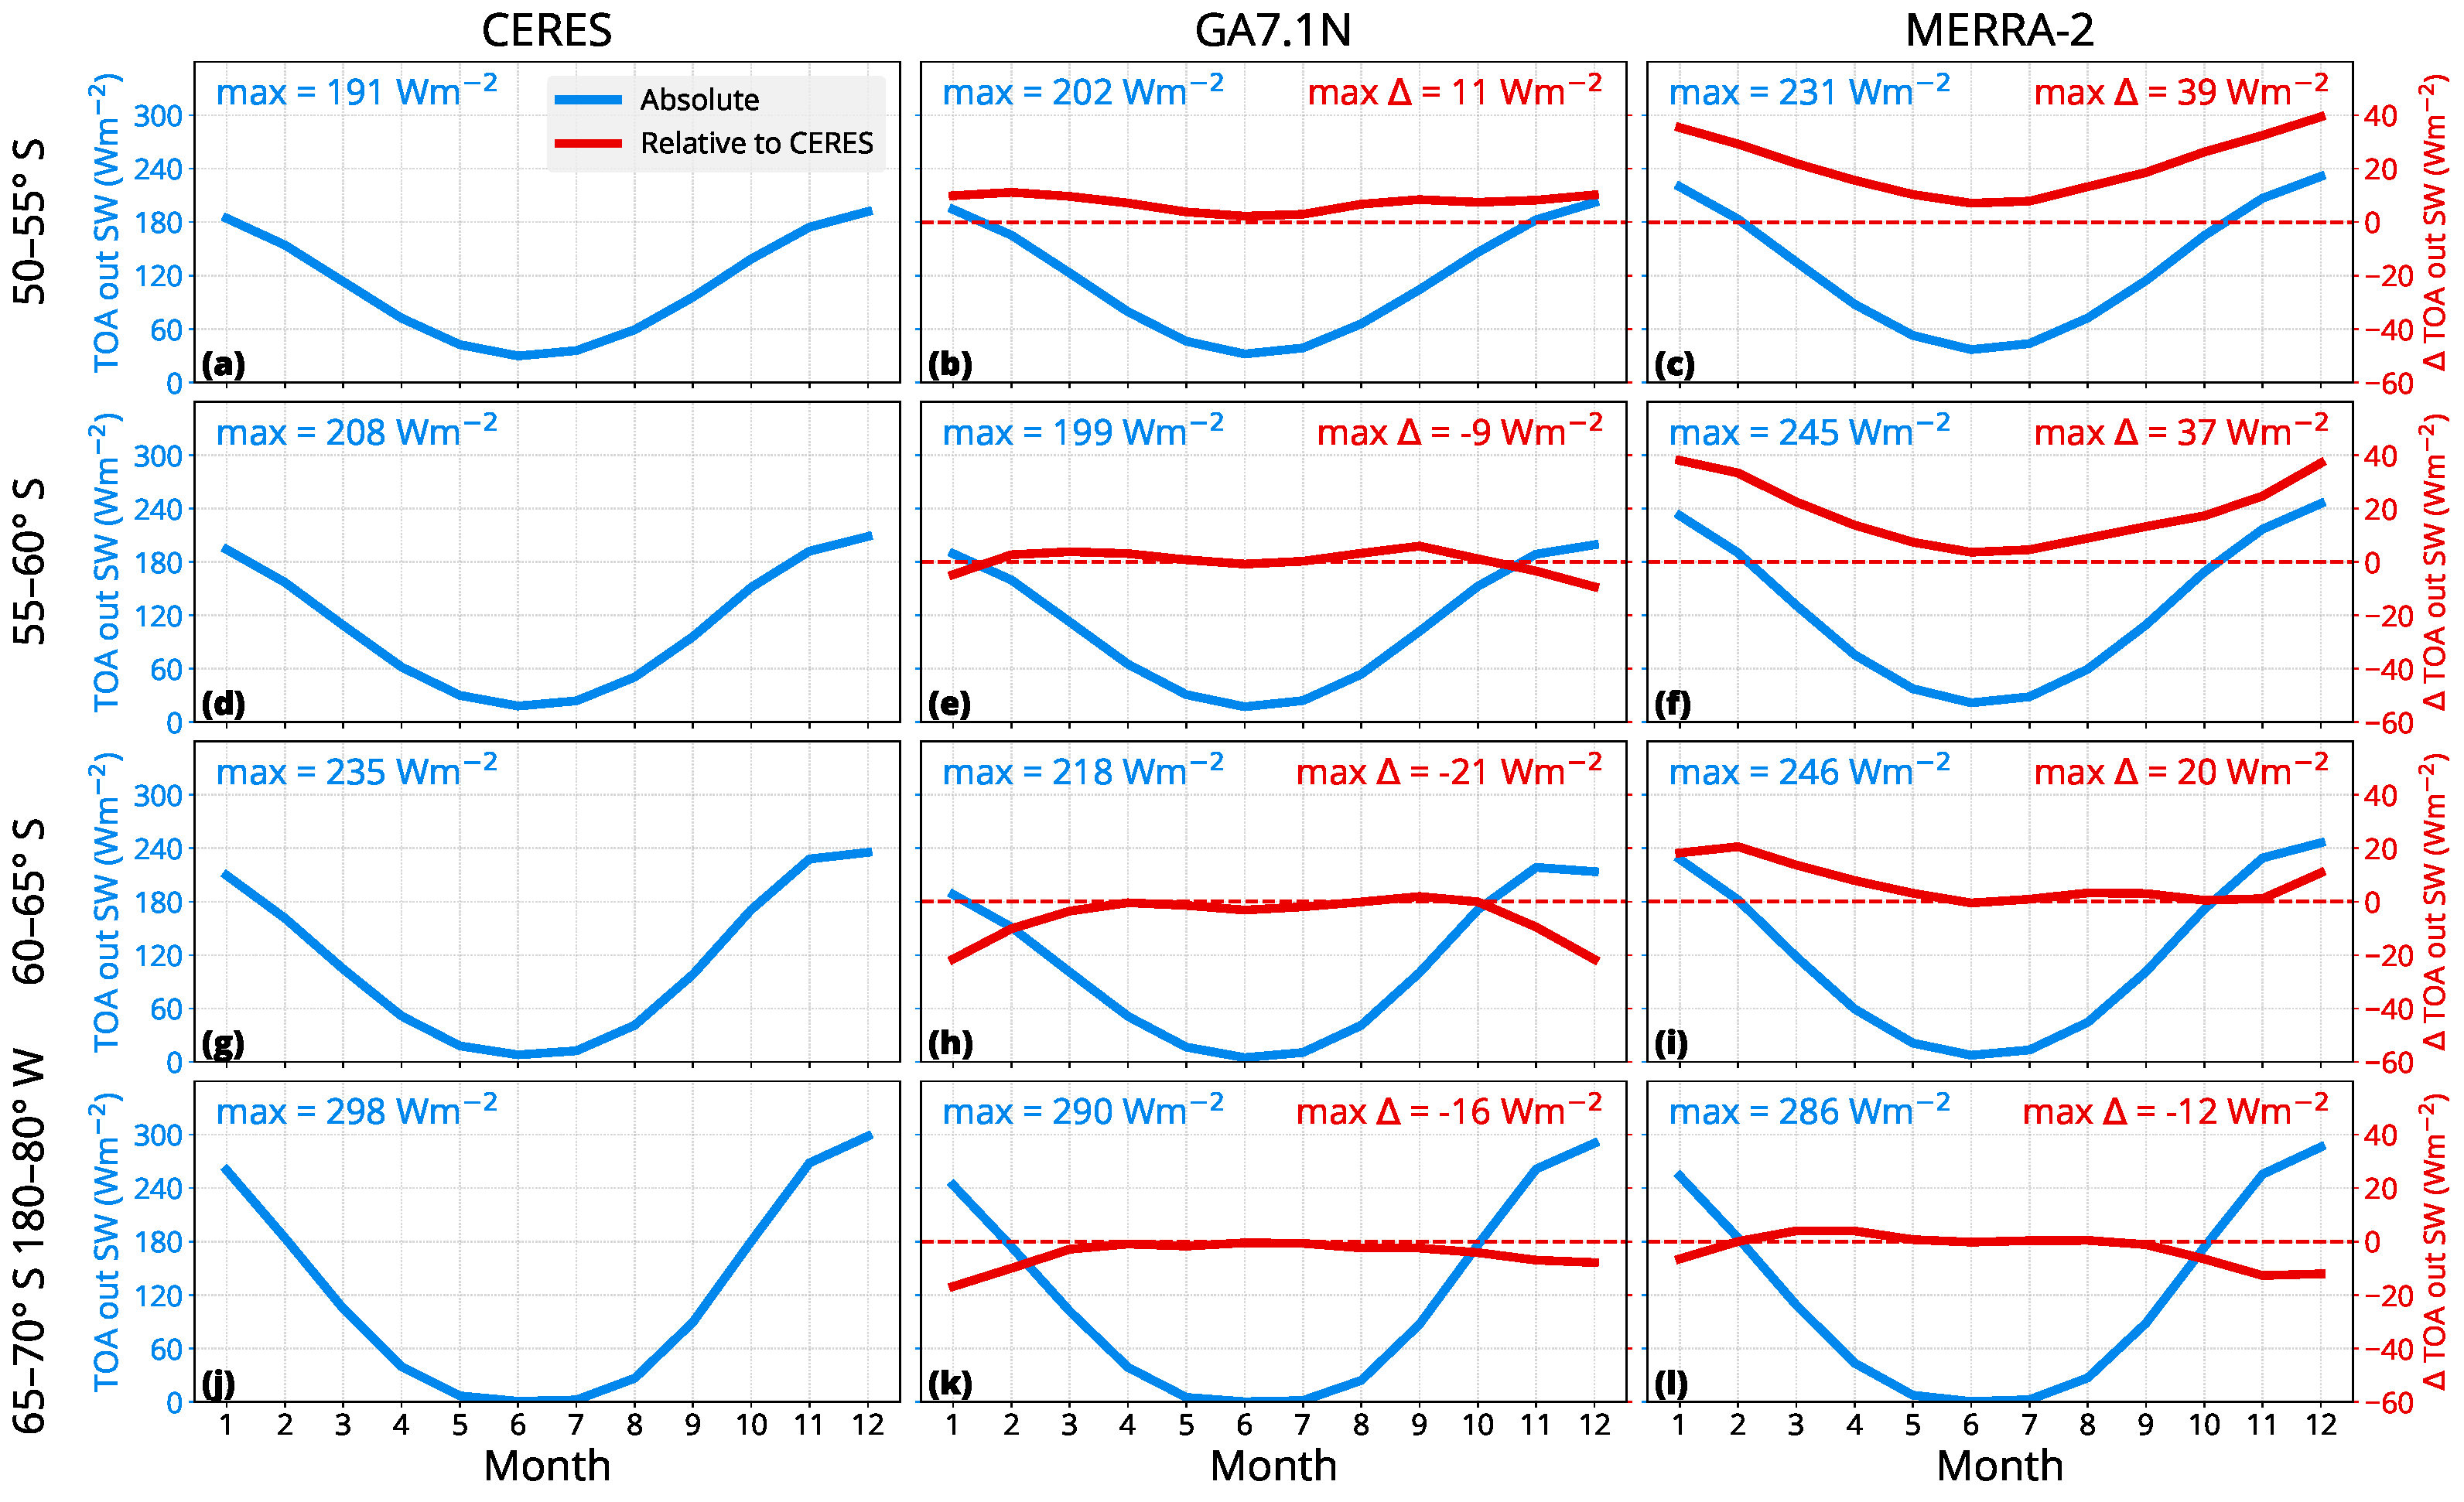
\includegraphics[width=1.12\textwidth]{chapter2/fig/sw_up_toa_time_rev1.pdf}}
\caption[Zonal means of the TOA outgoing SW radiation in CERES, GA7.1N and MERRA-2]{
Zonal means of the TOA outgoing SW radiation in CERES, GA7.1N and MERRA-2
during the years 2015--2018 in 5-degree latitude bands between 50 and
70$^\circ$S. The plots show monthly zonal mean TOA outgoing SW radiation
(blue) and its difference relative to CERES (red) as a function of month. Shown
are also the maxima ("max") and the difference from CERES ("max $\Delta$").
}
\label{fig:2:sw_up_toa_time}
\end{figure*}

Figure~\ref{fig:2:sw_up_toa_time} shows line plots of zonal mean reflected SW
radiation and bias relative to CERES by month in multiple latitude bands
between 50 and 70$^\circ$S, with the southernmost band 65--70$^\circ$S limited
to 180--80$^\circ$W to avoid covering land areas in Antarctica. The annual
cycle follows the expected seasonal pattern modulated by varying incoming solar
radiation with maxima of reflected radiation in December and maxima of bias in
December and January. The Antarctic sea ice extent, at its minimum in February
and peaking in September, is also likely a secondary modulating factor of the
TOA outgoing SW radiation at higher latitudes. The models represent the
seasonal pattern well, but differ substantially during the periods of peak
incoming solar radiation. The GA7.1N model (Fig.~\ref{fig:2:sw_up_toa_time}b, e,
h, k) exhibits bias ranging from $-$21 to +11 Wm$^{-2}$. The bias is positive
north of 55$^\circ$S and negative south of this latitude, with the greatest
absolute bias between 60 and 65$^\circ$S. MERRA-2 displays a clearly different
bias from GA7.1N, ranging from $-$12 to +39 Wm$^{-2}$ (Fig.
\ref{fig:2:sw_up_toa_time}c, f, i, l). The peak SW bias in MERRA-2 is positive for
latitudes north of 65$^\circ$S and negative south of this this latitude. The
absolute bias in MERRA-2 is much larger than in GA7.1N north of 60$^\circ$S and
similar to GA7.1N south of this latitude. Therefore, the MERRA-2 results are
valuable for contrasting with GA7.1. The strong latitudinal variation of the
TOA outgoing SW radiation bias is important to take into consideration.
Previous studies of SO clouds often did not discern different latitudes.

\begin{figure*}[t]
\centering
\centerline{\includegraphics[width=1.12\textwidth]{chapter2/fig/sw_bias_scatter_rev1.png}}
\caption[Scatter plot of SW radiation bias in GA7.1N and MERRA-2]{
Scatter plot of SW radiation bias in \textbf{(a)} GA7.1N and \textbf{(b)} MERRA-2 grid cells
between 55$^\circ$S and 70$^\circ$S in January 2018. Each point represents a
daily average of SW radiation bias as a function of near-surface air temperature
and near-surface relative humidity. The bias is expressed as a percentage of the
incoming solar radiation in the grid cell. The points are a random sample of
100000 points.
}
\label{fig:2:sw-bias-scatter}
\end{figure*}

\begin{figure*}[p]
\centering
\centerline{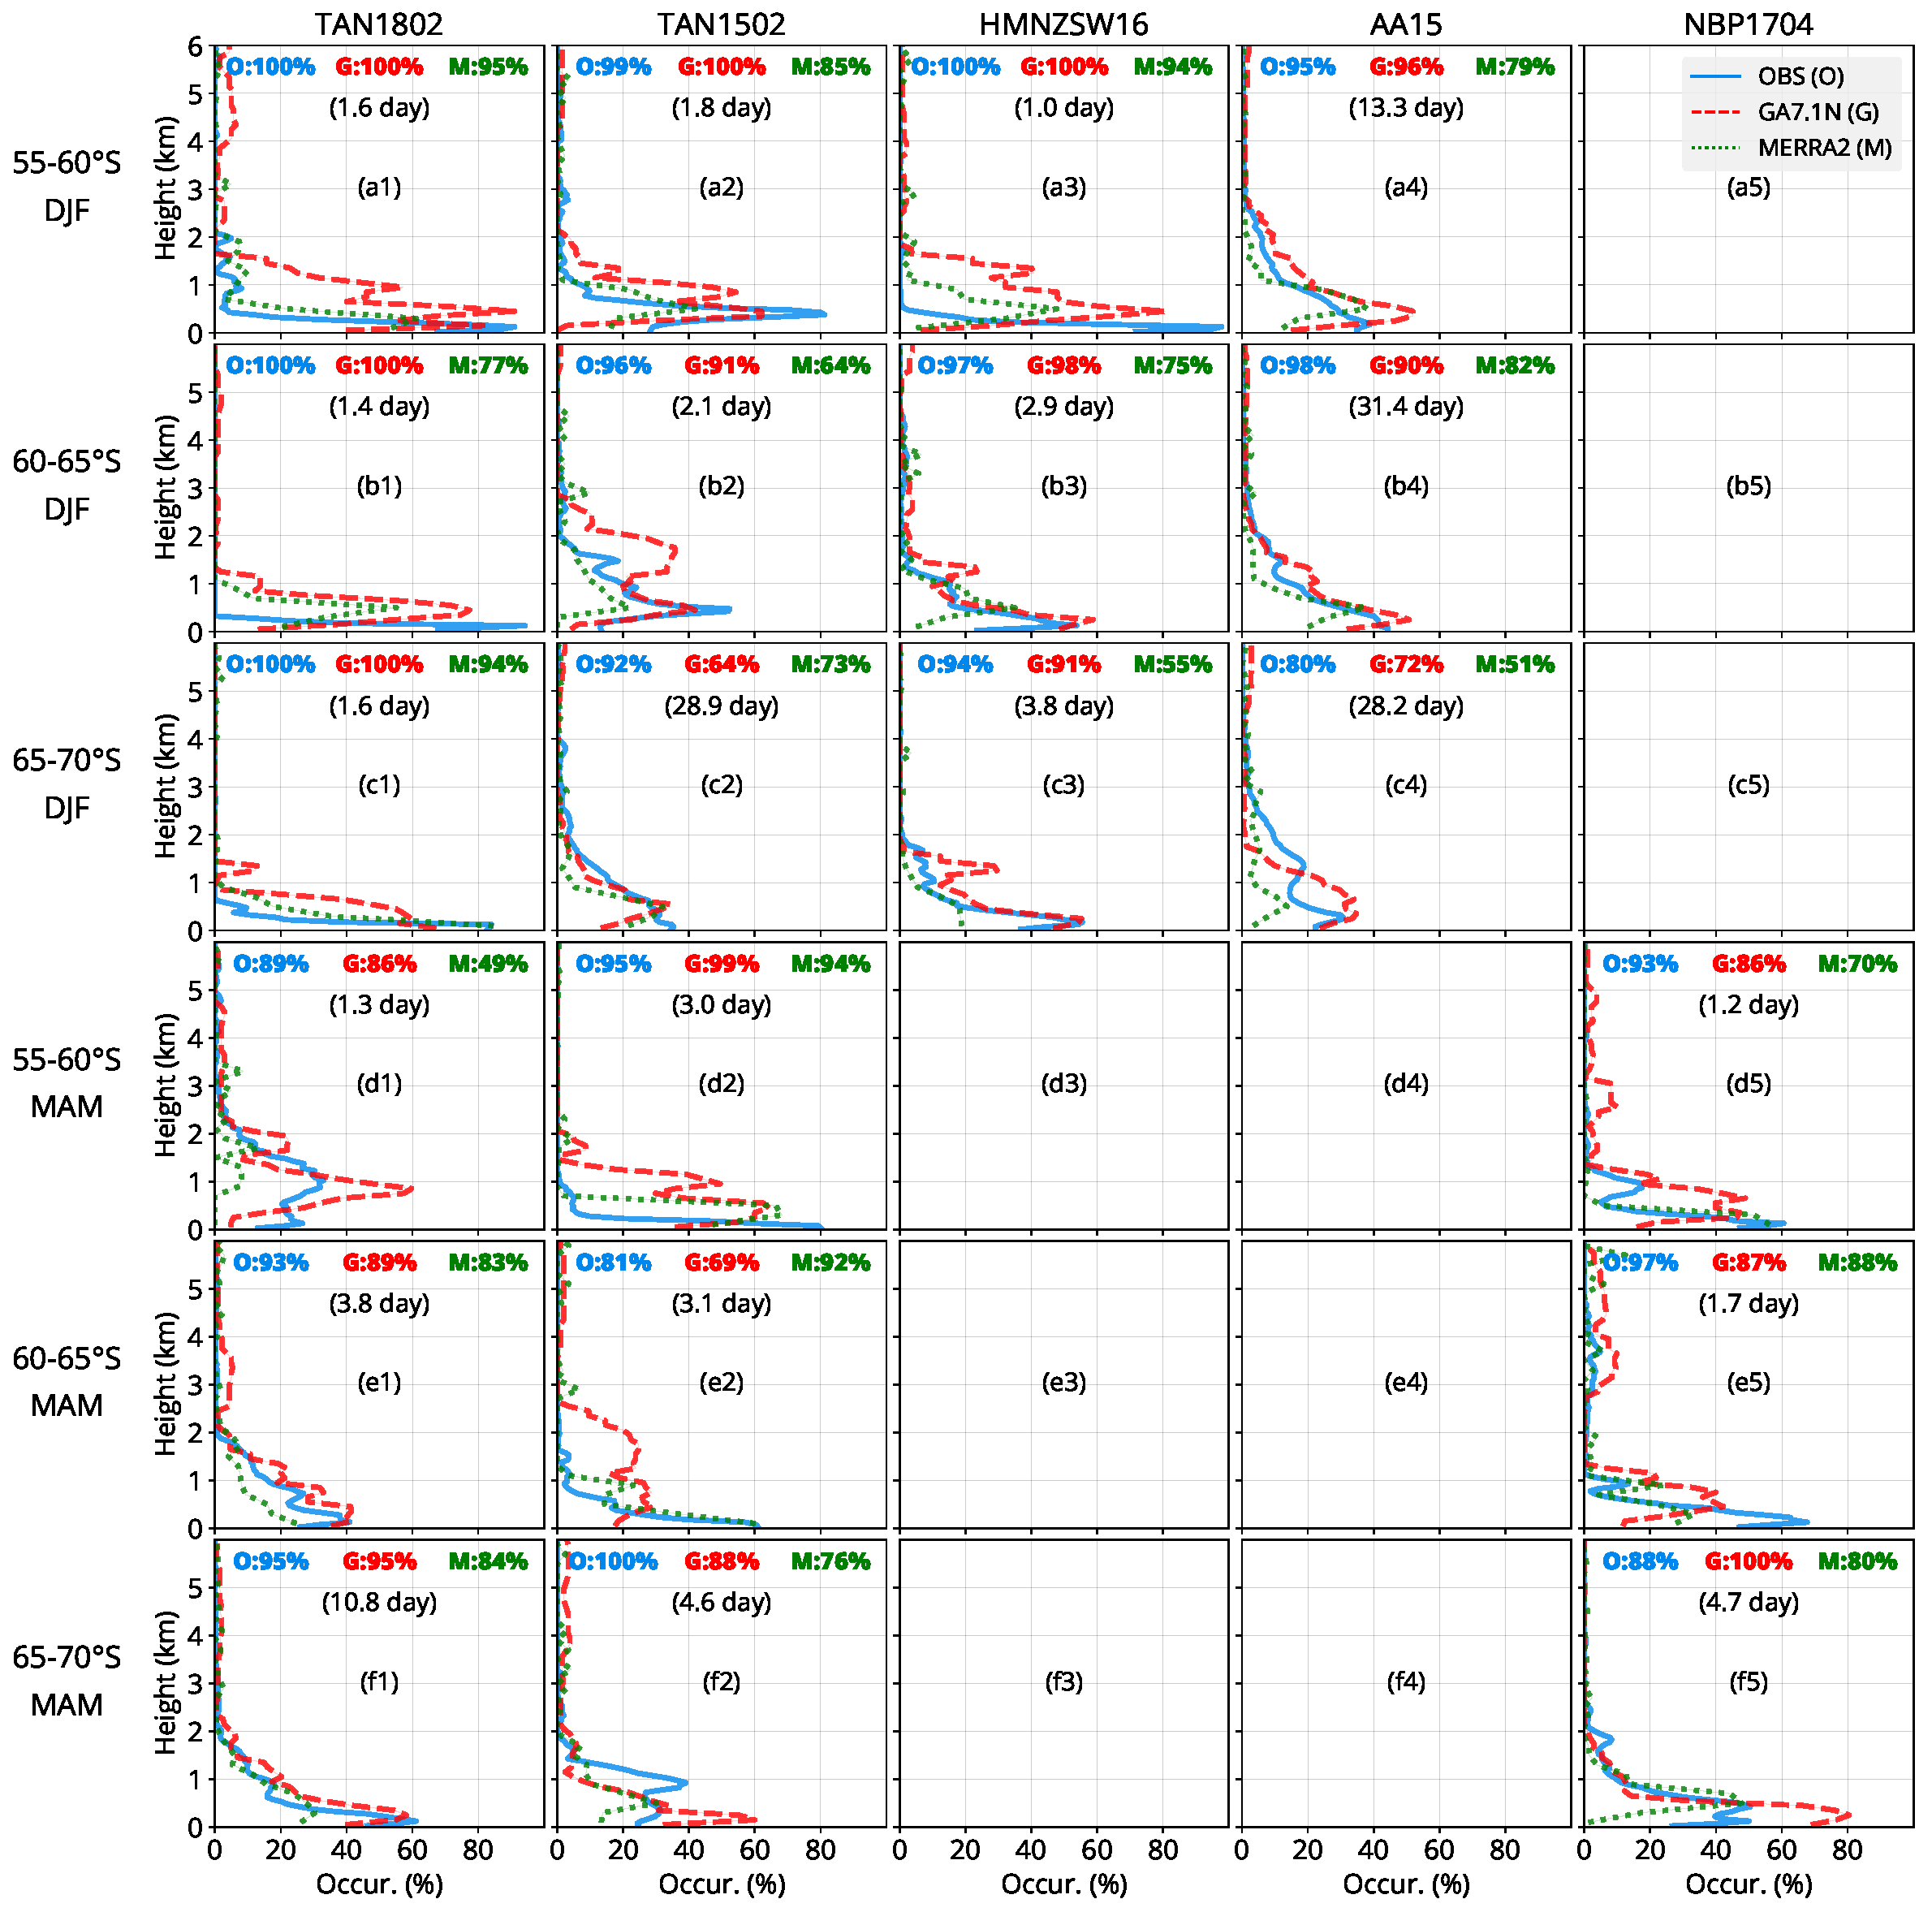
\includegraphics[width=1.12\textwidth]{chapter2/fig/cloud_occurrence_panel_rev1.pdf}}
\caption[Cloud occurrence frequency as a function of height derived from ceilometer
observations and model fields]{
Cloud occurrence frequency as a function of height derived from ceilometer
observations (OBS) and model fields (GA7.1N and MERRA-2). The observational and
model data were subsetted by latitude and season (DJF, MAM) along the voyage
track. The numbers at the top of each panel show total (vertically integrated)
cloud cover and the number of days the ship spent passing through the
spatiotemporal subset. The height in the plots is limited to 6 \unit{km}. There
was no significant amount of cloud detected above this level. The total cloud
cover is the fraction of profiles with at least one cloud masked range bin.
}
\label{fig:2:cloud-occurrence}
\end{figure*}

\begin{figure*}[t]
\centering
\centerline{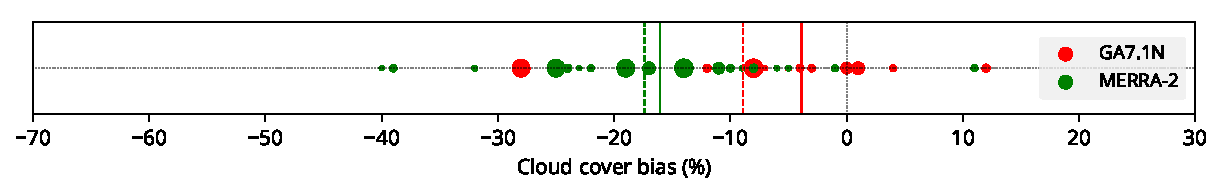
\includegraphics[width=1.12\textwidth]{chapter2/fig/cloud_cover_hist_rev1.pdf}}
\caption[Cloud cover bias in models relative to observations]{
Cloud cover bias in models relative to observations. The points represent
subsets as in Fig.~\ref{fig:2:cloud-occurrence}. The size of the circles is
proportional to the number of days of observations in the subset. The solid
lines are averages, and dashed lines are averages weighted by the number of days
the ship spent passing through the spatiotemporal subset.
}
\label{fig:2:cloud-cover-hist}
\end{figure*}

Figure~\ref{fig:2:sw-bias-scatter} shows scatter plot of the TOA outgoing SW
radiation bias in GA7.1N and MERRA-2 as a function of near-surface air
temperature and relative humidity between 55 and 70$^\circ$S in January
2018. The bias is predominantly negative in GA7.1N and positive MERRA-2. There
is a strong cluster of negative bias at temperature around 0$^\circ$C in
GA7.1N and $-$2$^\circ$C in MERRA-2, and a cluster of positive bias at higher
temperatures. This is consistent with the latitudinal dependence of bias in
both models shown above.

\subsection{Cloud occurrence in model and observations}
\label{sec:2:cloud-occurrence}

To understand how clouds contribute to the SW bias, we examine cloud cover and
cloud occurrence as a function of height in the models and observations. Figure
\ref{fig:2:cloud-occurrence} shows cloud occurrence profiles derived from
ceilometer observations on different voyages and GA7.1N and MERRA-2 model
output derived via the COSP surface lidar simulator, in subsets by latitude and
season. Most notably, the observed cloud cover is consistently very high in the
observations (80--100\%) for all periods and latitude bands examined and
greater than 90\% in most of the subsets. This finding differs substantially
from the modelled cloud cover derived via the surface lidar simulator, which
ranges between 69 and 100\% in GA7.1N, and is about 4--9\% lower than
observations across the subsets. The cloud cover in MERRA-2 is also lower than
observed and much lower than in GA7.1N, spanning 51--95\%. Only in 4 subsets is
the cloud cover greater in GA7.1N than observed, and only in 1 subset is the
cloud cover greater in MERRA-2 than observed (out of 21 subsets).  Our analysis
therefore shows that cloud cover is underestimated in both GA7.1N and MERRA-2
in the evaluated geographical regions and seasons.

Examination of the vertical distributions in Fig.~\ref{fig:2:cloud-occurrence}
shows that observations have a strong predominance of cloud below 2 \unit{km}
and peaking below 500 m in most subsets, including a substantial amount
of surface-level fog in some subsets. In contrast, GA7.1N and MERRA-2 simulate
clouds at a higher altitude, peaking at about 500 \unit{m} and generally the
peak is higher than in observed clouds. Especially, clouds below 500 m and fog
appear to be lacking in the models.

The subsets in Fig.~\ref{fig:2:cloud-occurrence} are derived from uneven
length of ship observations (1.0--28.9 days) due to the limited availability of data.
The longer subsets (Fig.~\ref{fig:2:cloud-occurrence}a4, b4, c2, c4, f1)
appear marginally more consistent between the models and observations
in terms of the cloud ocurrence profile, but the cloud cover is still markedly
underestimated.
Figure~\ref{fig:2:cloud-cover-hist} shows the model subsets of Fig.
\ref{fig:2:cloud-occurrence} as points by their cloud cover bias relative to
observations. It can be seen that GA7.1N underestimates cloud cover by about
4\% and MERRA-2 by 16\% when non-weighted averages are considered, and by 9\%
(GA7.1N) and 18\% (MERRA-2) when weighted averages are considered.
Due to the nature of the lidar measurements, middle to high clouds may be
obscured by low clouds, as the laser signal is quickly attenuated by thick
cloud. Therefore, the lack of clouds above 2 \unit{km} in the plots does not
imply that no clouds are present. The lidar simulator, however, ensures
unbiased 1:1 comparison with observations by accounting for the signal
attenuation.
The results demonstrate the value of surface cloud measurements in the SO
relative to satellite measurements such as CloudSat and CALIPSO, which would
likely provide a biased sample of these clouds because of "ground clutter"
and obscuration by higher-level clouds, respectively \citep{alexander2018}.

\subsection{Radiosonde observations}
\label{sec:2:radiosonde-observations}

We use radiosonde measurements performed on TAN1802 and NBP1704 to
evaluate boundary layer properties and correlate them with clouds observed by
a ceilometer. We compare the observations with "pseudo-radiosonde" profiles
extracted from model fields at the same location and time. The location is
based on the GNSS coordinates of the ship at the time of the balloon launch
(the ballon trajectory length was generally not long enough to span multiple
model grid cells in the lower troposphere).

We define a new quantity "SST lifting level" (SLL) derived
from SST and boundary layer atmospheric potential temperature,
defined as the level to which
an air parcel with the same temperature as SST, rising from the sea surface,
would rise adiabatically by buoyancy. That is, it is the level closest to the
surface at which potential temperature is equal to SST, provided the air parcel
is permitted to rise to this level by buoyancy (otherwise the air parcel does
not rise and SLL is 0 m). This quantitiy is applicable in sea ice-free
conditions in the SO, when cold Antarctic air is warmed by the open sea surface
and is lifted by buoyancy until it reaches a limit imposed by the atmospheric
stability of the atmosphere. Alongside the lifting condensation level (LCL) we
found SLL to be a useful quantity for evaluation of CBH. The
authors are not aware of any previous use of SLL, but this definition is
supported by observations (see below).

Apart from SLL and LCL, we also use the lower tropospheric stability (LTS)
\citep{klein1993}. LTS is defined as the difference between potential
temperature at 700 hPa and sea level pressure \citep{klein1993}. It has been
used in multiple previous studies
\citep{williams2006,franklin2013,williams2013,naud2014}. 

\begin{figure*}[p]
\centering
\centerline{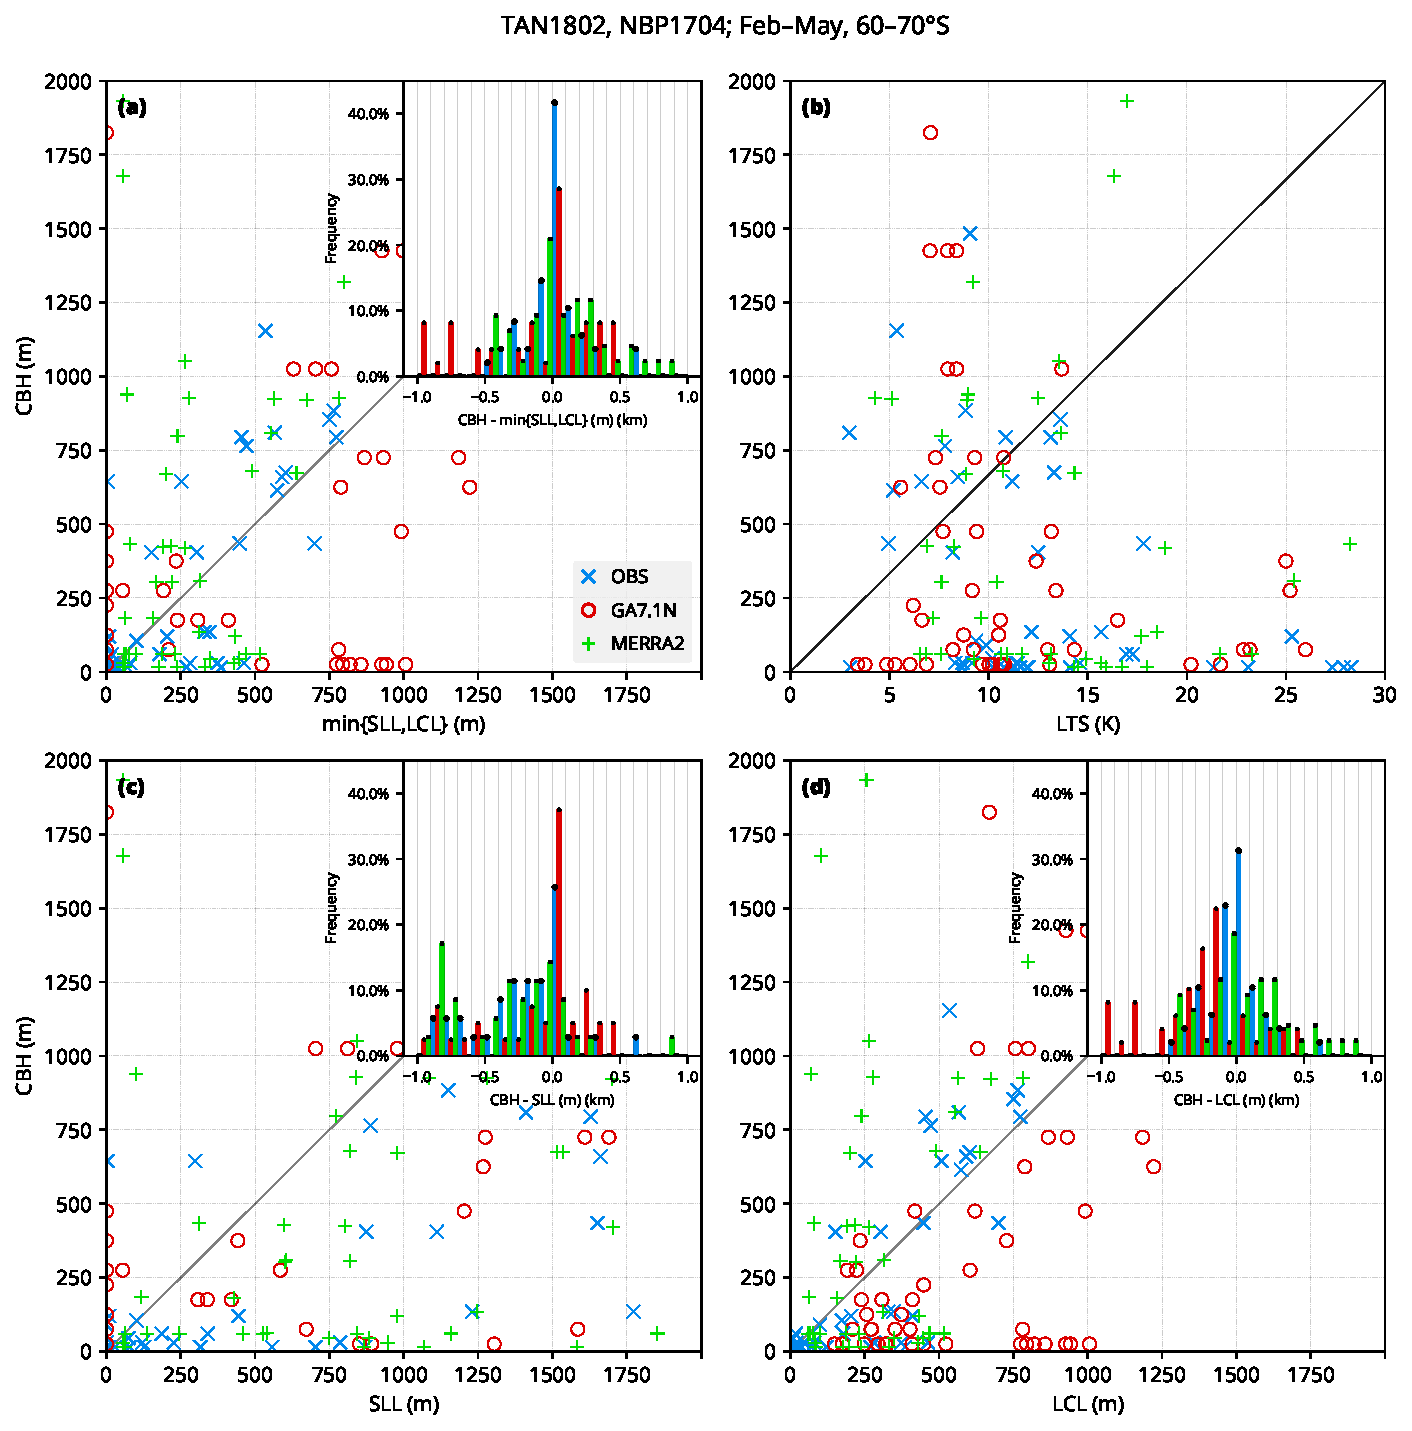
\includegraphics[width=1.12\textwidth]{chapter2/fig/rs_scatter_rev1.pdf}}
\caption[Scatter plots of radiosonde measurements on the TAN1802 and NBP1704 voyages]{
Scatter plots of radiosonde measurements on the TAN1802 and NBP1704 voyages
between February and May and 60--70$^\circ$S latitude. Corresponding profiles
from GA7.1N and MERRA-2 are selected, i.e. having the same geographical
coordinates and the same time of the year. Each point on the scatter plots
represents a radiosonde profile. The plots compare three datasets: observations
(OBS), GA7.1N and MERRA-2. The radiosonde observations are matched with
ceilometer (OBS) and COSP-based CBH (GA7.1N and MERRA-2). \textbf{(a)} shows the
points as a function of min\{SLL, LCL\} and CBH. The inset histogram shows
distribution of the difference of CBH and min\{SLL, LCL\} in bins of 100
\unit{m}, where each bin contains three bars for the three datasets.
\textbf{(b, c, d)} show the points as a function of LTS, SLL and LCL,
respectively.
}
\label{fig:2:rs-scatter}
\end{figure*}

Figure~\ref{fig:2:rs-scatter} shows the observed and modelled relationship
between CBH and the minimum of SLL and LCL ("min\{SLL,LCL\}"), LTS, SLL and
LCL. A large fraction of the observed points (OBS) in Fig.
\ref{fig:2:rs-scatter}a lie close to the origin (40\% in the first 100 m in
observations, vs.~26\% and 17\% in GA7.1N and MERRA-2, respectively), which
suggests that near zero min\{SLL,LCL\} is a good indicator of fog or very low
cloud, a relationship not well-represented in the models. The remaining
observed points show a close equivalence between min\{SLL,LCL\} and CBH, while
the models do not represent this equivalence well.  The histogram in Fig.
\ref{fig:2:rs-scatter}a reveals that about 42\% of observed profiles have CBH
within 100 \unit{m} of min\{SLL,LCL\}, while only about 28\% of GA7.1N and 21\%
of MERRA-2 profiles do.

Using SLL or LCL as a predictor for CBH individually resulted in a weaker
relationship than min\{SLL,LCL\}: 25\% and 31\% of OBS profiles have CBH within
100 \unit{m} of SLL and LCL, respectively (Fig.~\ref{fig:2:rs-scatter}c, d).
This suggests that min\{SLL,LCL\} is more strongly related to CBH than SLL or LCL
individually. Figure~\ref{fig:2:rs-scatter}b shows CBH as a function of LTS. LTS
does not display a good predictive ability for CBH in this dataset, with the
exception of very stable profiles (LTS > 15 K), when observed CBH was below 250
\unit{m} in all but one case.

\begin{figure*}[p]
\centering
\centerline{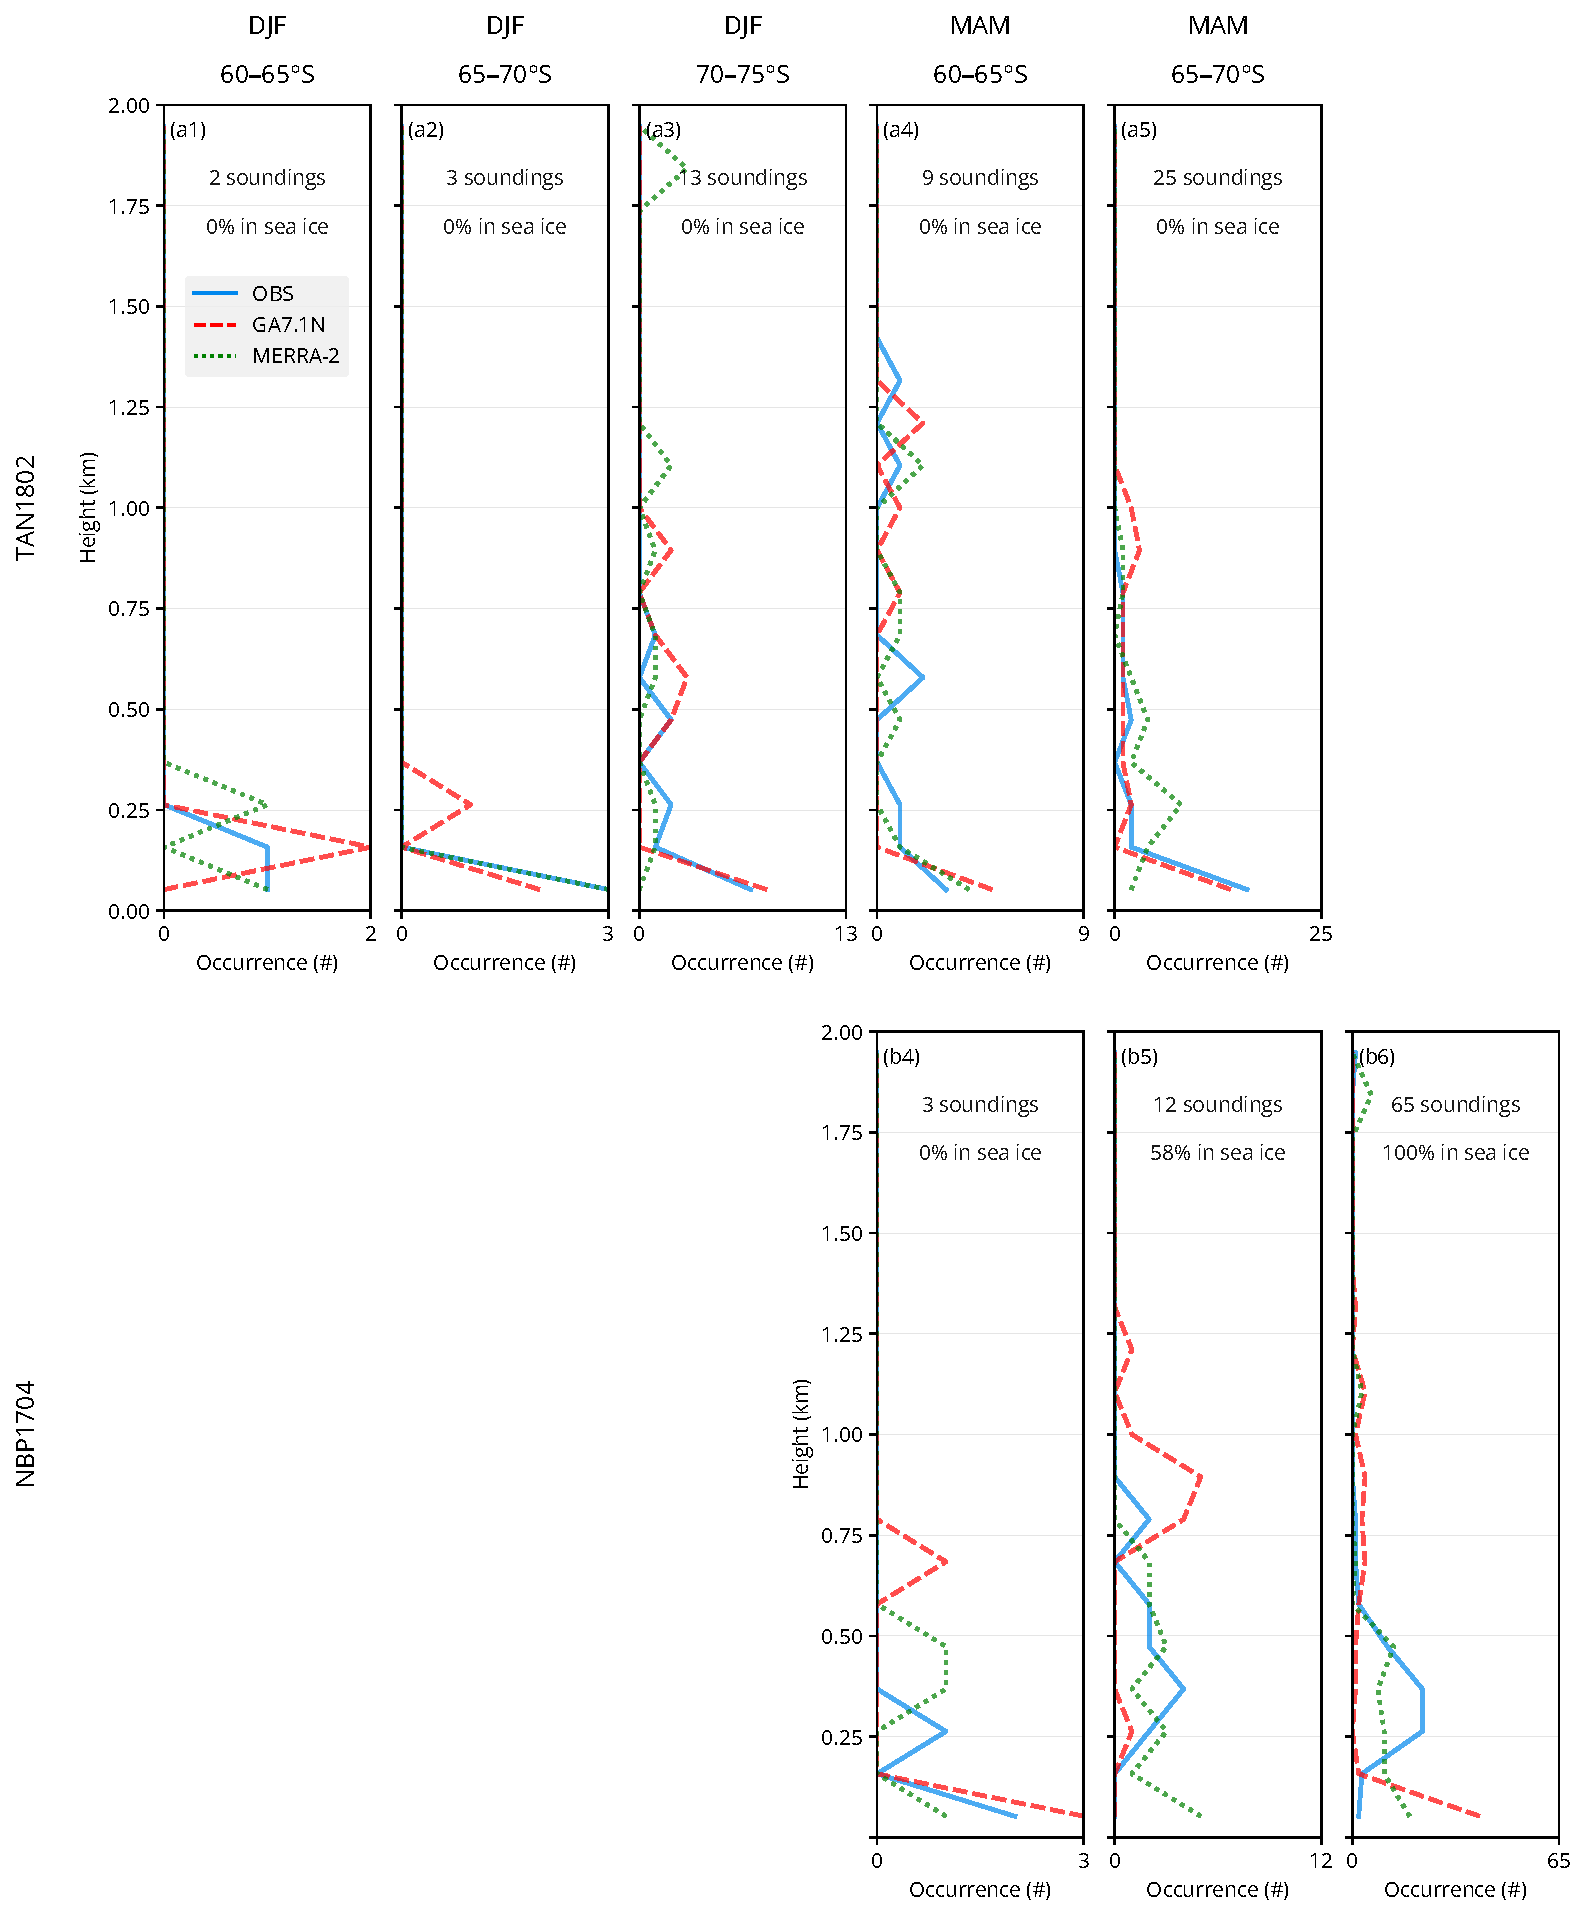
\includegraphics[width=1.12\textwidth]{chapter2/fig/sst_lifting_level_panel_rev3.pdf}}
\caption[Number of occurrences of min\{SLL,LCL\} by height]{
Number of occurrences of min\{SLL,LCL\} by height
derived from radiosonde observations (OBS) on
TAN1802 and NBP1704, and the equivalent profiles in GA7.1N and MERRA-2.  Shown
are subsets by latitude between 60 and 75$^\circ$S and seasons DJF and MAM.
The numbers at the top of each panel indicate the number of profiles which make
up the histogram and the percentage of sea ice cases determined from NSIDC
satellite-derived sea ice concentration.
}
\label{fig:2:sll-distribution}
\end{figure*}

Figure~\ref{fig:2:sll-distribution} shows the distribution of min\{SLL,LCL\}
derived from radiosonde observations and model fields. In observations, the
quantity almost consistently peaks near the ground and reaches up to 1.5 km in
ice-free cases (Fig.~\ref{fig:2:sll-distribution}a1--a5, b4). GA7.1N represents
this distribution relatively well. This is not the case with MERRA-2, which is
less likely to peak near the ground (Fig.~\ref{fig:2:sll-distribution}a3, a5, c4).
The sea-ice cases (Fig.~\ref{fig:2:sll-distribution}b5, b6)
show markedly different observed distribution of the quantity, with peak at
about 300 m.  GA7.1N and MERRA-2 represent the distribution over sea ice
relatively poorely.

\begin{figure*}[p]
\centering
\centerline{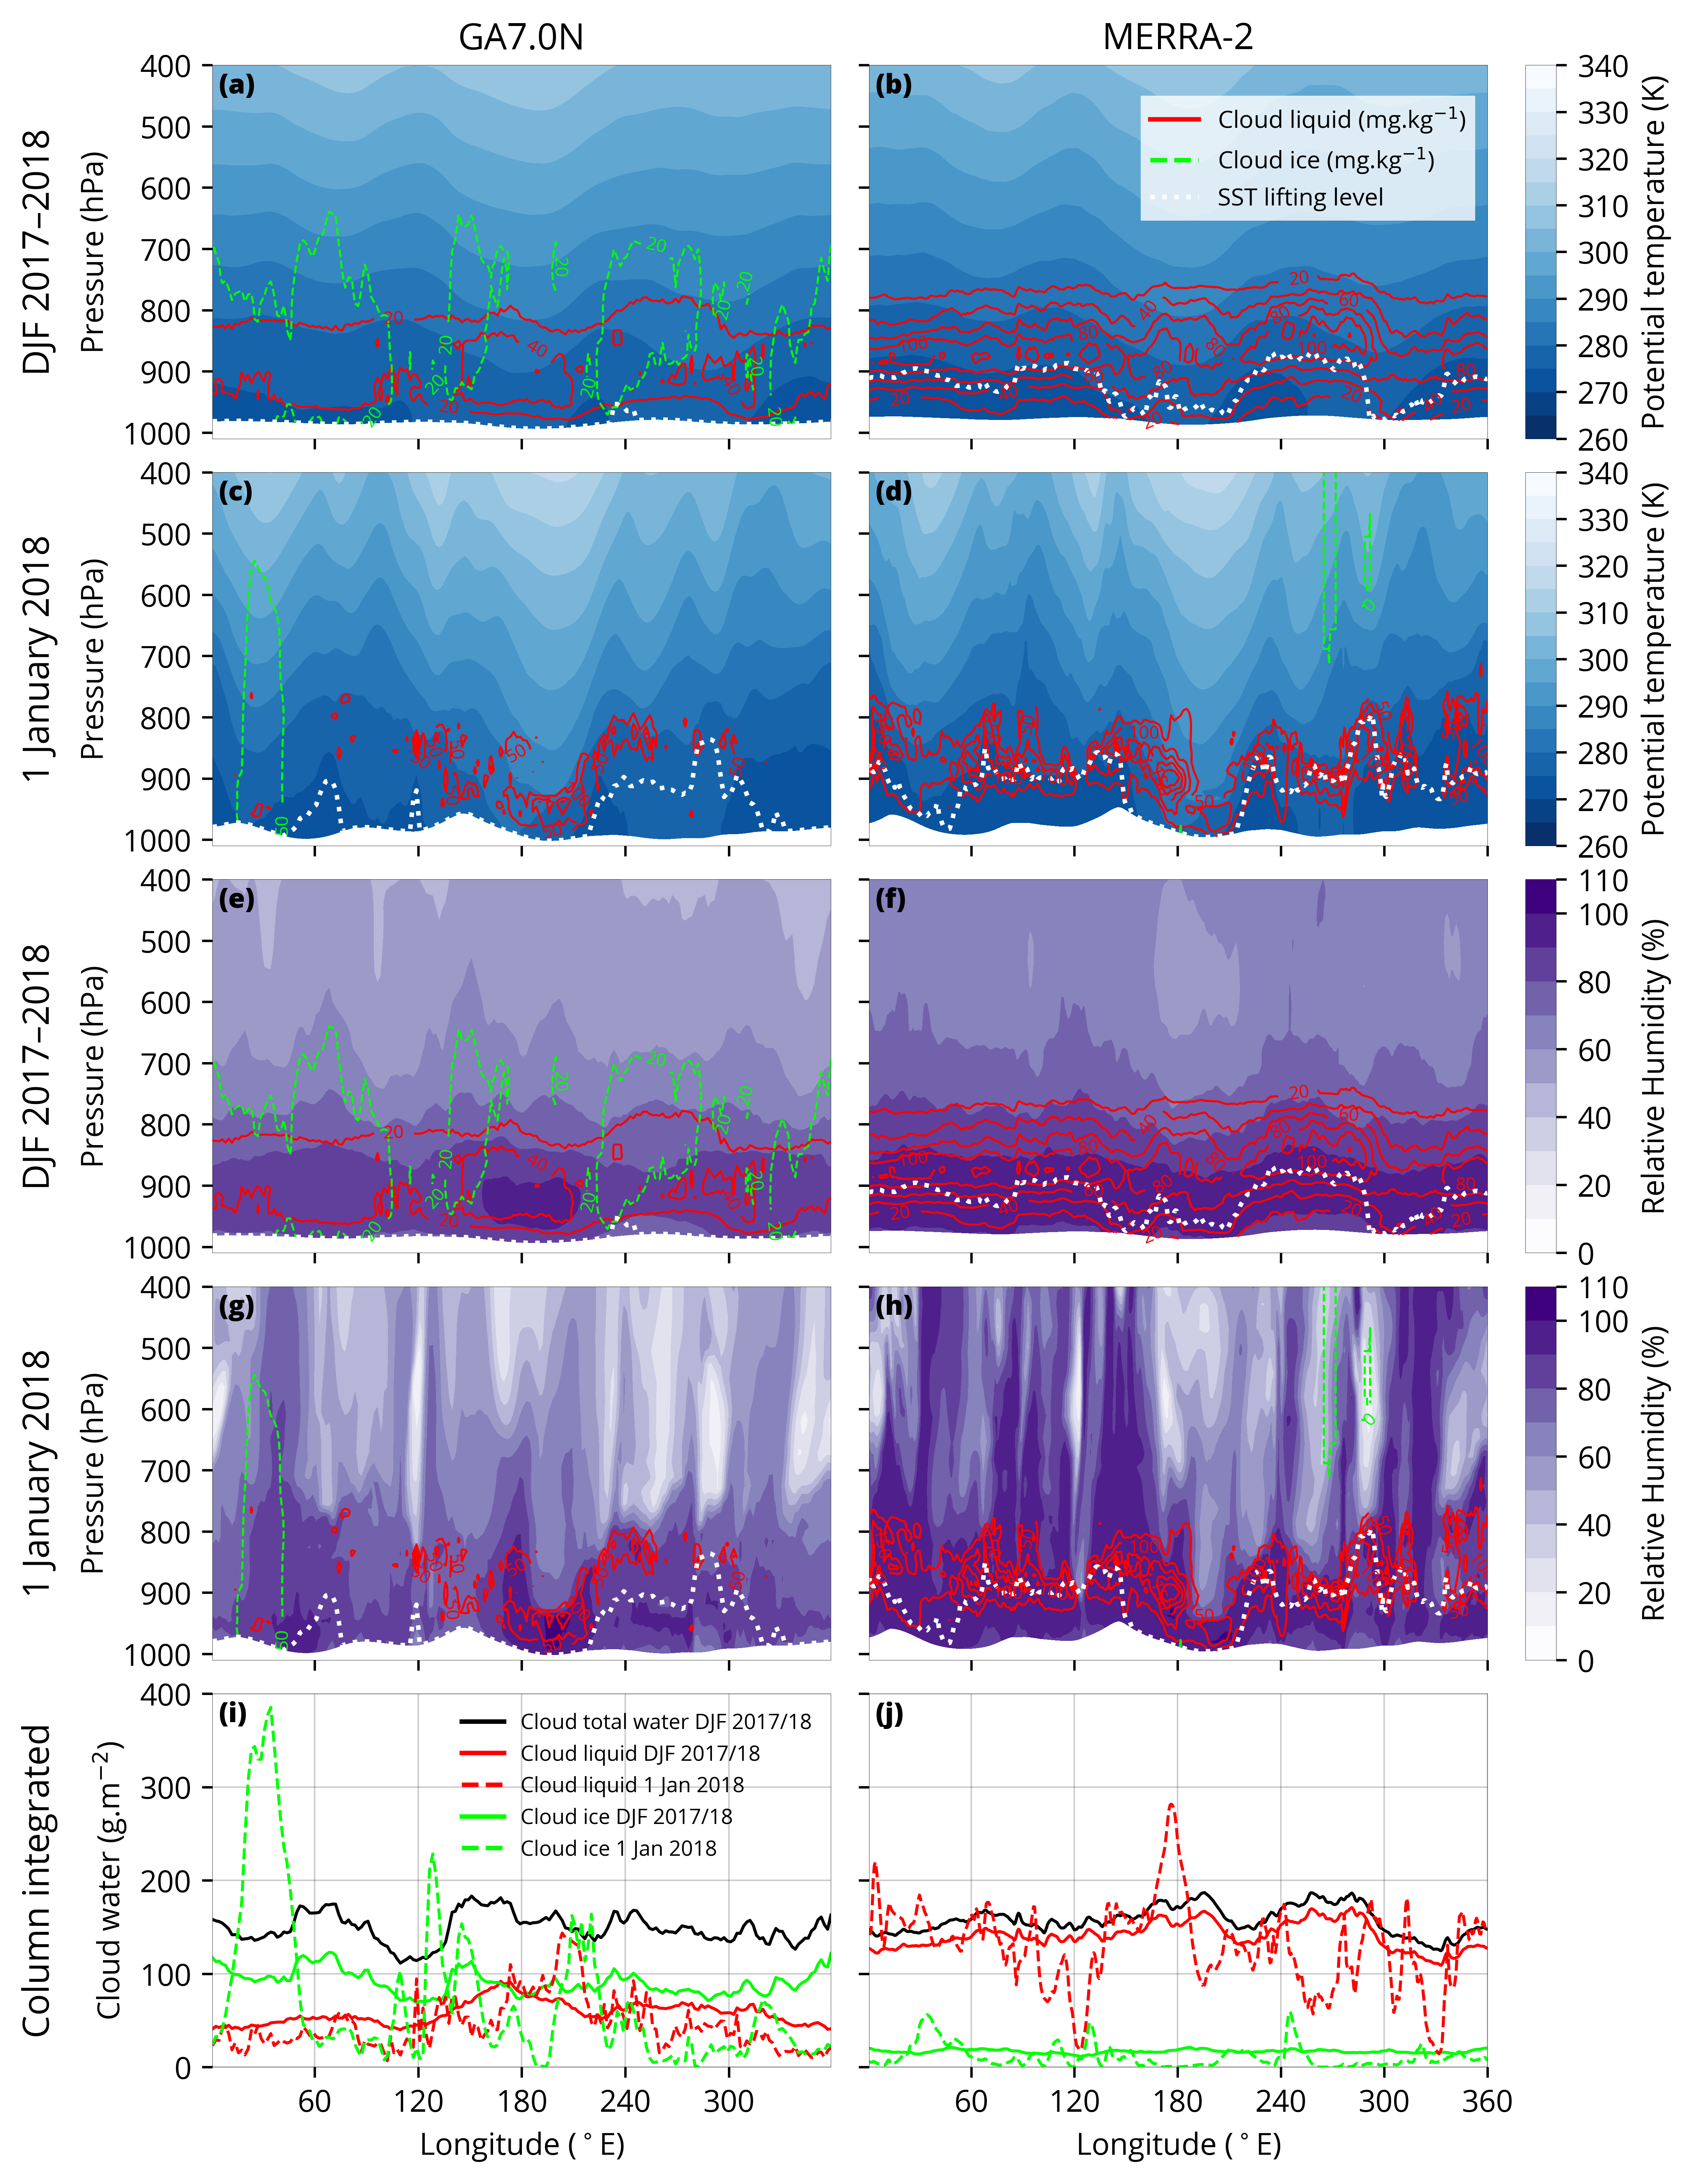
\includegraphics[width=\textwidth]{chapter2/fig/zone_panel_rev2.png}}
\caption[Zonal plane plot of cloud liquid and ice mixing ratios in GA7.1N and MERRA-2 at
60$^\circ$S]{
Zonal plane plot of cloud liquid and ice mixing ratios in GA7.1N and MERRA-2 at
60$^\circ$S. The cloud liquid and ice mixing ratios are plotted as contours on
top of the potential temperature fields \textbf{(a--d)} and relative humidity
fields \textbf{(e--h)}. SLL is indicated by a white line. \textbf{(a, b, e, f)}
show a seasonal average in DJF 2017/2018 and \textbf{(c, d, g, h)}
show a daily average on 1 January 2018. \textbf{(i, j)} show the
column-integrated values of cloud liquid and ice water as a function of
longitude corresponding to the plots above. All liquid shown in the plots
is supercooled (air temperature is less than 0$^\circ$C everywhere).
}
\label{fig:2:zone-panel}
\end{figure*}

\subsection{Zonal plane comparison of GA7.1N and MERRA-2}
\label{sec:2:zonal-plane-comparison}

In order to better understand the differences in the SW radiation bias between
GA7.1N and MERRA-2, we inspect zonal plane plots of cloud occurrence and
thermodynamic fields of the models in DJF 2017/18 and 1 January 2018 (Fig.
\ref{fig:2:zone-panel}). The figure shows seasonal and daily average cloud liquid
and ice mixing ratio contours plotted over two different backgrounds --
potential temperature and relative humidity (RH). The daily average plots
(Fig.~\ref{fig:2:zone-panel}c, d) show a very pronounced difference between
the cloud liquid amount between the two models, with MERRA-2 simulating a much
greater amount of cloud liquid. In contrast, GA7.1N simulates cloud with ice,
which are nearly absent in MERRA-2 at the chosen contour levels. The liquid
content is generally concentrated near SLL in MERRA-2, but much less so in GA7.1N,
where SLL is often at 0 m. The cloud ice in GA7.1N generally has significantly
greater vertical extent than the cloud liquid. These differences are also
present on the seasonal scale (Fig.~\ref{fig:2:zone-panel}a, b). The difference
in potential temperature between the models is relatively small. GA7.1N, however,
shows a slightly higher potential temperature.
The RH field is very different between GA7.1N and MERRA-2, with MERRA-2
simulating higher RH by about 10\%.

Pehaps most interestngly, the vertically integrated liquid and ice content
(Fig.~\ref{fig:2:zone-panel}i, j) is very different between the models. Both
models simulate almost the same liquid + ice total, but the phase composition
of cloud in GA7.1N is majority ice, while in MERRA-2 it is almost entirely
liquid.

\section{Discussion}

The TOA outgoing SW radiation assessment shows that the models exhibit monthly
average biases of up to 39 \unit{W m^{-2}} (MERRA-2, 50--55$^\circ$S in
December), and that these biases have a significant latitudinal dependency,
with the opposite sign of bias between different latitude bands. In GA7.1N the
bias is predominantly negative, while in MERRA-2 the bias is predominanly
positive. Similar pattern of bias is present in both models. The bias is positive
north of 55$^\circ$S (65$^\circ$S) in GA7.1N (MERRA-2) and negative south of
this latitude.
This finding is consistent with \cite{schuddeboom2019}, who observed opposite
sign of SW cloud radiative effect south and north of 55$^\circ$S in GA7.1.

A very similar geographical pattern of bias is present in DJF and
MAM, suggesting that similar cloud biases are present in both seasons. This
is also supported by Fig.~\ref{fig:2:cloud-occurrence}, which does not display
a significant difference in observed cloud occurrence and bias in the models
between DJF and MAM.  Consistent with the maximum of incoming solar radiation,
December and January were found to be the months with the greatest absolute
bias in the models. Therefore, fixing the representation of clouds in the SO
in these months is relatively more important than in other months.

Figure~\ref{fig:2:sw-bias-scatter} suggests that the bias correlates not only
with latitude, but also with near-surface air temperature. The negative bias
is strongly clustered around 0$^\circ$C in GA7.1N, and $-$2$^\circ$C in
MERRA-2, and positive bias is predominantly correlated with higher temperature.

The ship-based lidar cloud occurrence revealed close to 100\% cloud cover in
multiple subsets. Subsetting allowed us to identify whether the cloud cover is
substantially different by latitude and season, and also sample independent
weather situations (it is expected that cloud occurrence profiles are highly
correlated over several days due to persistance of synoptic situations). The
subsets show a relatively consistent cloud occurrence profile peaking below 500
m, and almost zero above 2 km. This is possibly also due to
obscuration of lidar signal by lower clouds, a fact which is also accounted
for by the lidar simulator and therefore unbiased in the comparison.
The models generally do not
reproduce this profile well. Apart from underestimating the total cloud cover,
the peak of cloud occurrence in the models is higher than observed. Improving
the cloud profile representation in the models is likely key for improving the
SW radiation bias.

The effect of clouds on SW radiation is the product of cloud cover (the
fraction of the sky containing clouds) and cloud albedo (the fraction of SW
radiation reflected by the clouds). With our ship-based lidar observations we
measured cloud cover (total, and cloud cover as a function of height), while we
did not measure cloud albedo. The cloud cover was almost consistently
underestimated in both GA7.1N and MERRA-2 across all latitudes. At the same
time, the satellite observations show that MERRA-2 reflects too much all-sky SW
radiation. Therefore, the cloud albedo in MERRA-2 must be too high in order to
cause too much all-sky SW radiation reflection despite the lack of cloud cover.
This effect is visible on the daily scale in Fig.
\ref{fig:2:sw_up_toa_geo}j--l, where the individual clouds in MERRA-2 appear
significantly brighter than on satellite observations.

Remarkably, the observed cloud ocurrence profiles appear
to be similar between the DJF and MAM seasons and
latitude bands between 55 and 70$^\circ$S (Fig.~\ref{fig:2:cloud-occurrence}):
if we focus on the subsets with more than 10 days (Fig.~\ref{fig:2:cloud-occurrence}a4, b4, c2, c4, f1),
i.e. not heavily skewed toward a single weather situation,
we find that they are
all characterised by a peak below 500 m of 25--60\% and falling to near-zero
above 2--3 km, sometimes with a minor secondary peak between 1 and 2 km.
The simulated profiles show a slightly higher altitude of the primary peak
between 0 and 1 km, underestimated in MERRA-2 by up about two thirds,
falling to near-zero between 2 and 3 km, without any substantial secondary peak.
The total cloud fraction appears to be more strongly underestimated at high
latitudes in GA7.1N in DJF, by 8--28\% (Fig.~\ref{fig:2:cloud-occurrence}c2, c4)
vs.~8\% (Fig.~\ref{fig:2:cloud-occurrence}b4).
This is an important consideration in connection with the SW radiation bias, which shows a strong
latitudinal gradient of the TOA outgoing SW radiation bias in the models
(Fig.~\ref{fig:2:sw_up_toa_geo},~\ref{fig:2:sw_up_toa_time}). Based on the the
presented results a plausible explanation for the SW radiation bias could be
overestimation of cloud albedo north of about 55$^\circ$S (65$^\circ$S) in
GA7.1N (MERRA-2) causing positive TOA outgoing SW radiation bias north of this
latitude and underestimation of cloud cover over the whole SO causing negative
TOA outgoing SW radiation bias south of this latitude.
We should note that some of the observations in the latitude band 65--70$^\circ$S
include time periods when the ships were docking at the station. These periods
could be affected by continental Antarctic flow, see for example \cite{jolly2018}.

Precipitation is currently not implemented in the lidar simulator. In lidar
observations, the cloud masking algorithm used does not discern precipitation
and cloud. Therefore, cloud occurrence in simulated lidar profiles can be biased
to lower values relative to observations if substantial amounts of precipitation
occurred during the time period. We tested this effect by eliminating profiles
affected by precipitation as detected by a co-located
Metek Micro Rain Radar version 2 (MRR-2) on the TAN1802 voyage and found
relatively little difference in the cloud occurrence profiles.

In the ship observations we found a notable correspondence between CBH, SLL and
LCL. Boundary layer thermodynamics, determining the lifting levels, is a
plausible driver of cloud formation in the absence of other forcing. We
examined SLL in models and radiosonde observations, and found differences which
are likely too small to explain the cloud occurrence differences between the
models and ceilometer observations. \cite{bodas-salcedo2012}, in their analysis
of an earlier version of the GA model (GA3.0) using cyclone composites also
noted that biases in thermodynamics are not likely to explain the SW radiation
bias, but may still play a significant role. The presence of positive TOA
outgoing SW radiation bias in the SO between 50 and 55$^\circ$S in GA7.1, which
contrasts with the negative bias south of the latitude, is important because it
places a limit on the applicability of other studies which used SO
observational data from regions north of 55$^\circ$S \citep{lang2018}.

In Section~\ref{sec:2:radiosonde-observations} we show that min\{SLL,LCL\} has a
stronger equivalence to CBH than SLL, LCL individually or LTS.  This
relationship becomes quite notable when examining the individual voyage
radiosonde profiles (not presented here). We hypothesise that the theoretical
reason for this relationship is the following. When SLL is higher than LCL, an
air parcel warmed by the sea surface to temperature close to SST rises by
buoyancy past LCL to a level with the equivalent potential temperature.  The
water vapour starts to condensate at LCL (assuming enough cloud condensation
nuclei are present at 100\% saturation), forming cloud with CBH equal to LCL.
If SLL is lower than LCL, the air parcel rises to the level of equivalent
potential temperature, where air lifted from the sea surface eventually
accumulates, potentially forming cloud if enough moisture is transported from
the sea surface. The models do not represent the observed relationship well (see also Chapter 4),
and improving this relationship may be one way of improving the cloud
simulation.

Considering the strong observed relationship between min\{SLL,LCL\} and CBH
(CBH tends to occur at the same level as min\{SLL,LCL\}), we evaluated the
distribution of min\{SLL,LCL\} in the models in comparison with radiosonde
observations (Fig.~\ref{fig:2:sll-distribution}). We found that GA7.1N
represents this distribution relatively well in sea-ice-free cases, while
MERRA-2 underestimates cases when min\{SLL,LCL\} was near the surface. This may
be the reason for the underestimation of very low cloud and fog in this model
identified in the comparison with lidar observations. Therefore, improving the
distribution of the quantity in MERRA-2 may lead to improvement of low cloud
simulation.
In the period of our observations, SST in MERRA-2 MERRA-2 is based on the \cite{donlon2012}
dataset \citep{gelaro2017}. The accuracy of SST in this dataset is 0.57 K.
This could potentially contribute to the boundary layer biases identified here.

It is interesting to contrast our results with previous studies which used
cyclone compositing for the TOA SW radiation bias evaluation in GCMs. We cannot
make substantial conclusions from our results on how much of the model bias is
attributable to cyclones. It appears, however, that the cloud cover and cloud
liquid and ice mixing ratio bias in GA7.1N is systematic rather than isolated to
cyclonic activities due to its relative consistency across spatiotemporal
subsets in the high latitude SO. This does not rule out even greater biases
related to cyclonic sectors. Specifically, \cite{bodas-salcedo2014} evaluated a
large set of models, including HadGEM2-A, a predecessor model to HadGEM3,
likely affected by similar biases, and found that about 80\% of grid cells
south of 55$^\circ$S could be classified as affected by a cyclone, and that
these grid cells were responsible for the majority of the total SW radiation
bias.  Moreover, their cyclone compositing showed that the bias in HadGEM2-A
was largely negative in the cold quadrants, and near zero in the warm
quadrants.  Their results also indicate a strong contrast in SW bias south and
north of 55$^\circ$S, similar to the result we found in GA7.1N.  We think these
results can be reconciled with our study by assuming that the model has a
particular difficulty in representing cloud in situations when near-surface air
temperature is lower than the SST. In these regions the heat flux is from the
ocean to the atmosphere is positive, which in the austral summer predominantly
occur south of 55$^\circ$S and in the cold sectors of cyclones. The cloud
representation when near-surface air temperature is greater than SST is
relatively more accurate, this case occurring predominantly north of
55$^\circ$S and in the warm sector of cyclones.  As shown in Fig.
\ref{fig:2:sw-bias-scatter}, the negative TOA outgoing SW radiation bias in the
models is clustered at zero and sub-zero temperatures. This suggests a
possible explanation that sub-zero air mass advecting from Antarctica or from
sea ice covered areas over warm water (cold-air outbreaks) could be inducing low cloud and fog, and
this process is not well represented in the models \citep{bodas-salcedo2012}.

Previous studies have documented that supercooled liquid is often present in
the SO cloud in summer months \citep{morrison2011,huang2012,chubb2013,huang2016,bodas-salcedo2016,jolly2018,listowski2019}. We cannot substantially add to these findings
with our observations, although preliminary analysis of a polarising lidar
Sigma Space MiniMPL profiles from the TAN1802 voyage suggests supercooled
liquid was commonly present in the ubiquitous stratocumulus cloud. The
side-by-side comparison of cloud liquid and ice mixing ratios on the zonal
plane (Fig.~\ref{fig:2:zone-panel}) suggests that models can differ
significantly in their representation of cloud phase, with GA7.1N simulating
markedly less supercooled liquid than MERRA-2. This is the most likely
the explanation for the overestimation of TOA outgoing SW radiation in MERRA-2,
despite the underestimated cloud cover in this model. If cloud cover is
increased in MERRA-2 to better match with the lidar observations, the cloud
albedo would have to be lowered to obtain a reasonable match of TOA outgoing SW
radiation with CERES.

The 2016--2018 voyages may have been affected by the unusually low sea ice
extent (discussed below), which can have a significant effect on cloud
\citep{frey2018,taylor2015}. The modulating effect of sea ice on cloud in the
SO has previously been shown by \cite{listowski2019} and there is an apparent
difference in cloud between the Ross Sea and Ross Ice Shelf as shown by
\cite{jolly2018}, with cloud over the ice shelf having smaller cloud cover, a
greater amount of altostratus cloud and a smaller amount of deep convective
cloud. The sea ice and ice shelves block transport of heat and moisture to the
atmosphere. Their low thermal conductivity and high albedo mean the surface can
cool to very low temperature and thus have an effect on the radiation balance
of the atmosphere. We did not focus on sea ice conditions, since one can expect
the effect of cloud biases on the SW radiation bias over sea ice to be small --
the ice surface is already highly reflective in the SW, and the presence of
cloud has little impact on the grid cell SW reflectivity (the SW albedo of
cloud is similar to sea ice, depending on the sea ice concentration).

The Antarctic sea ice extent has undergone a rapid decrease starting in the
spring of 2016 after about a decade of slightly increasing extent
\citep{turner2017,stuecker2017,doddridge2017,kusahara2018,schlosser2018,ludescher2018}.
The sea ice extent due to this decrease was found to be the lowest on
observational record since 1979, and the Ross Sea was particularly affected by
this anomaly. The unusually low sea ice extent likely affected atmospheric
observations made on the voyages presented in this study, e.g. the TAN1802
voyage in February and March 2018 to the Ross Sea experienced no sea ice during
the entire voyage. Because sea ice is an important factor influencing the
atmospheric boundary-layer stability and radiation balance, a significant
secondary effect on cloud cover, cloud phase and opacity is expected. Sea ice
is, however, not expected to be responsible for the SO SW radiation bias described
here, because the bias is present even when sea ice concentration is
prescribed from satellite observations, as is the case in the nudged run GA7.1
and the MERRA-2 reanalysis. Given that few of the ship-based
observations were collected before 2016, we cannot reliably estimate how
the anomalous sea ice extent affected our results. 

In our results we found that even when model atmospheric dynamics is
nudged to a reanalysis
based on past observations, the TOA outgoing SW radiation bias is large and
cloud occurrence, especially of low cloud and fog, is underestimated. CBH is
found to be strongly linked to the boundary layer thermodynamics, and this link
does not seem to be well represented in GA7.1N and MERRA-2. We therefore expect
that cloud and boundary layer parametrisations (as part of subgrid scale
processes in the models) are responsible for this bias. We have identified
parts of the GA7.1N model most likely responsible: the large-scale cloud scheme,
the prognostic cloud fraction and prognostic condensate scheme (PC2) scheme \citep{wilson2008a,wilson2008b} and the boundary layer scheme. A
future study should focus on these schemes to identify the parts responsible
for the bias. In particular, the model should improve simulation of very low
cloud and fog and achieve a closer match between the lifting levels and CBH
(Fig.~\ref{fig:2:rs-scatter}a).

\begin{table*}[t]
\caption[A table showing a "back-of-the-envelope" calculation]{
A table showing a "back-of-the-envelope" calculation how the GA7.1N peak TOA
outgoing SW radiation bias (Fig.~\ref{fig:2:sw_up_toa_time}) would change if
the cloud cover were increased by 5\% (Fig.~\ref{fig:2:cloud-cover-hist}),
asssuming the cloud albedo does not change. The "corrected" TOA outgoing SW
radiation is calculated by multiplying the original value by 1.05.
}
\label{tab:2:bias-correction}
\centering
\centerline{\scalebox{0.8}{
\begin{tabular}[t]{lcccc}
\hline
Latitude & TOA out. SW at max. $\Delta$ (Wm$^{-2}$) & Max. $\Delta$ TOA out. SW (Wm$^{-2}$) & Corrected Max. $\Delta$ TOA out. SW (Wm$^{-2}$) & Explained error \\
\hline
55--60$^\circ$S & 199 & -9 & 0.95 & 111\% \\
60--65$^\circ$S & 214 & -21 & -10.3 & 51\% \\
65--70$^\circ$S & 243 & -16 & 3.85 & 76\% \\
\hline
\end{tabular}
}}
\end{table*}

In Table~\ref{tab:2:bias-correction} we present a simple calculation how the
GA7.1N peak TOA outgoing SW radiation bias would change if the cloud cover were
increased by 5\% (as suggested by Fig.~\ref{fig:2:cloud-cover-hist}), assuming
the cloud albedo does not change. This correction would explain 51--111\% of
the bias depending on the latitude. The remaining part of the bias must be
attributed to cloud albedo. One way this could be improved is by increasing the
supercooled liquid fraction, or by increasing the total cloud water (liquid +
ice) path. Therefore, our results suggest that in GA7.1N underestimation of
cloud cover is responsible for the majority of the negative TOA outgoing SW
radiation bias, relative to underestimation of cloud albedo.

\section{Conclusions}

We analysed 4 years of observational SO ship data, and contrasted them with a
nudged run of the GA7.1 GCM, and MERRA-2 reanalysis. We used satellite
observations of the Earth radiation budget to assess the TOA outgoing SW
radiation bias in the SO in the models. We examined the total cloud cover and
vertical distribution of cloud as measured by ceilometers and simulated by a
ceilometer simulator based on the model data. We also compared SO radiosonde
observations from two voyages with pseudo-radiosonde profiles from the models in
order to assess boundary layer stability and the correlation between cloud base
and atmospheric lifting levels. We also compared model fields of cloud liquid
and ice content, potential temperature and relative humidity in a zonal plane
analysis across the SO to contrast cloud and thermodynamics simulated
by GA7.1N and MERRA-2.

The SO SW radiation bias is significant in GA7.1N and MERRA-2, and tends to be
positive in the northern parts of the SO and negative in the southern parts of
the SO in both models. MERRA-2 shows greater absolute bias than GA7.1N. SO
ship-based lidar and radiosonde observations are a valuable tool for model cloud
evaluation, considering the amount of low cloud in this region which is likely
poorly sampled by satellite instruments due to possible obscuration by higher
overlapping cloud. The main findings of this study are that multi-year
ship-based observations:

\begin{itemize}
\item corroborate satellite-based evidence of underestimated cloud cover, with
both GA7.1N and MERRA-2 underestimating cloud cover on average by about 4--9\%
(GA7.1N) and 18\% (MERRA-2),
\item show that low cloud below 2 \unit{km} is almost continuous in the SO in
summer months in sea ice-free conditions, and not well represented in the
models,
\item indicate that boundary layer thermodynamics is a strong driver of cloud in
the SO, and this relationship is not well represented in the models,
\item suggest that subgrid-scale processes in situations when near-surface
atmospheric temperature is lower or close to SST are responsible for the cloud
misrepresentation.
\end{itemize}

Here, we introduced a new quantity (a thermodynamic level) called SST lifting
level (SLL), which is the level of neutral buoyancy of an adiabatically lifted
parcel with temperature equal to SST. The motivation for introducing this level
was the frequently observed occurrence of cloud base at this height, together with
LCL. We think that this is explained by the strongly thermodynamically-driven
cloud in the Soutern Ocean boundary layer and is linked to the particular
conditions of the summertime Southern Ocean: sub-zero temperature of the
near-surface atmosphere, destabilised by the relatively warmer (near-zero)
sea surface.

Future studies of SO cloud representation in the GA model could focus on
specific details of the model subgrid-scale cloud processes (such as the large
scale cloud, boundary layer and convection schemes), and how their tuning
impacts cloud occurrence distributions compared to the ship observations. The
stark difference between GA7.1N and MERRA-2 cloud liquid and ice content also
remains to be explained, and could provide valuable insight for improving the
SO SW radiation bias in the model and the reanalysis.

\clearpage

\fontsize{10pt}{12pt}
\sffamily

\subsection*{Code and data availability}

The original COSP version 1 simulator is open source and available publicly at
\url{https://github.com/CFMIP/COSPv1}. The modified COSP version 1 simulator
including the ground-based lidar simulator used in this study is open source and
available at \url{https://alcf-lidar.github.io}. The cl2nc
software for converting Vaisala CL51 data to NetCDF is available at
\url{https://github.com/peterkuma/cl2nc}. The CERES EBAF and SYN1deg products
are available publicly from the CERES website:
\url{https://ceres.larc.nasa.gov/}. The Neal-Real-Time DMPS SSMIS Daily Polar
Gridded Sea Ice Concentrations product is available publicly from the NSIDC
website: \url{https://nsidc.org/data/nsidc-0081}. The Hadley Centre Sea Ice and
Sea Surface Temperature data set (HadISST) is available publicly from the Met
Office website: \url{https://www.metoffice.gov.uk/hadobs/hadisst/}. The MERRA-2
data are available publicly from the MERRA-2 website:
\url{https://gmao.gsfc.nasa.gov/reanalysis/MERRA-2/}. The ship-based
observations dataset as well as all processing code is available on request
from the authors.

\subsection*{Author contributions}

Peter Kuma participated on methodology development, voyage observations, data
analysis, writing and reviewing of the manuscript. Adrian McDonald participated
on conceptualisation, funding acquisition, methodology development, voyage
observations, data analysis, writing and reviewing of the manuscript. Olaf
Morgenstern participated on model development, methodology development, data
analysis, writing and reviewing of the manuscript. Simon Alexander, John
Cassano, Jamie Halla, Sean Hartery, Sally Garrett, Mike Harvey, Simon Parsons,
and Graeme Plank participated on voyage observations and reviewing of the
manuscript. Vidya Varma and Jonny Williams participated on model development
and reviewing of the manuscript.

\subsection*{Acknowledgements}

We would like to thank everyone who participated on obtaining the Southern
Ocean voyage observations, especially Kelly Schick and Peter Guest for
performing ceilometer and radiosonde measurements on RV \textit{Nathaniel B.
Palmer}; the Royal New Zealand Navy for ceilometer and radar measurements on
HMNZS \textit{Wellington}; Alex Schuddeboom for deployment of instruments on RV
\textit{Nathaniel B. Palmer}, the crew of the TAN1502, \textit{Aurora
Australis} V1--V3 2015/16, HMNZS \textit{Wellington}, NBP1704 and TAN1802
voyages.  Logistical and technical support for the ceilometer observations made
aboard \textit{Aurora Australis} during the summer of 2015/16 were provided as
part of the Australian Antarctic Science project 4292. We acknowledge the Met
Office for use of the MetUM, and for providing the HadGEM3 model. We
acknowledge NASA-GMAO and ECMWF for the MERRA-2 and ERA-Interim reanalyses,
respectively. In this analysis we used publicly available satellite datasets
provided by NASA and NSIDC. The CERES data were obtained from the NASA Langley
Research Center CERES ordering tool (\url{https://ceres.larc.nasa.gov}). We
wish to acknowledge the contribution of the NeSI high-performance computing
facilities to the results of this research. New Zealand's national facilities
are provided by the NZ eScience Infrastructure and funded jointly by NeSI's
collaborator institutions and through the Ministry of Business, Innovation \&
Employment's Research Infrastructure programme (\url{https://www.nesi.org.nz}).
We would like to acknowledge the financial support that made this work possible
provided by the Deep South National Science Challenge via the "Clouds and
Aerosols" project.  We acknowledge the software tools Python, R \citep{r},
numpy \citep{oliphant2006}, scipy \citep{scipy}, matplotlib \citep{hunter2007},
Climate Data Operators (CDO) \citep{schulzweida2018} and parallel
\citep{tange2011}, which we used in our data analysis.

\normalsize
\normalfont
